% An attributed exposition derived from OpenAI, September 24, 2026.
% Modified for this exposition; the source argument is licensed Apache-2.0.
\documentclass[11pt,a4paper]{article}
\usepackage[T1]{fontenc}
\usepackage[utf8]{inputenc}
\usepackage{lmodern}
\usepackage[margin=1in]{geometry}
\usepackage{amsmath,amssymb,amsthm,mathtools}
\usepackage{microtype,booktabs,array,enumitem}
\usepackage{flafter}
\usepackage[section]{placeins}
\usepackage[numbers,sort&compress]{natbib}
\usepackage{xcolor,tikz}
\usepackage{xurl}
\usetikzlibrary{arrows.meta,positioning,calc,patterns}
\definecolor{linkblue}{RGB}{25,60,98}
\usepackage[colorlinks=true,linkcolor=linkblue,citecolor=linkblue,urlcolor=linkblue,
 bookmarksnumbered=true,pdfusetitle,unicode]{hyperref}
\usepackage[nameinlink,capitalise,noabbrev]{cleveref}
\urlstyle{same}
\pdfgentounicode=1
\pdfinfoomitdate=1
\pdftrailerid{}
\pdfsuppressptexinfo=15
\newtheorem{theorem}{Theorem}[section]
\newtheorem{lemma}[theorem]{Lemma}
\newtheorem{proposition}[theorem]{Proposition}
\newtheorem{corollary}[theorem]{Corollary}
\theoremstyle{definition}
\newtheorem{definition}[theorem]{Definition}
\theoremstyle{remark}
\newtheorem{remark}[theorem]{Remark}
\newcommand{\R}{\mathbb R}
\newcommand{\C}{\mathbb C}
\newcommand{\N}{\mathbb N}
\newcommand{\Z}{\mathbb Z}
\newcommand{\dd}{\mathrm d}
\newcommand{\eps}{\varepsilon}
\newcommand{\Id}{\mathrm{Id}}
\DeclareMathOperator{\Op}{Op}
\DeclareMathOperator{\supp}{supp}
\DeclareMathOperator{\tr}{tr}
\DeclareMathOperator{\dist}{dist}
\DeclareMathOperator{\vol}{vol}
\DeclareMathOperator{\diag}{diag}
\DeclareMathOperator{\rank}{rank}
\numberwithin{equation}{section}
\setcounter{tocdepth}{2}
\setlength{\emergencystretch}{2em}
\setlist{topsep=4pt,itemsep=3pt}
\renewcommand{\bibfont}{\raggedright}
\allowdisplaybreaks[2]
\raggedbottom
\clubpenalty=10000
\widowpenalty=10000

\title{An exposition of smooth anisotropic Calder\'on uniqueness\newline
from full boundary data}
\author{Kaiwen Jin\thanks{\href{mailto:yui.ui.siki@gmail.com}{yui.ui.siki@gmail.com}}}
\date{October 12, 2026}
\hypersetup{pdftitle={An exposition of smooth anisotropic Calderon uniqueness from full boundary data},
 pdfauthor={Kaiwen Jin}}
\begin{document}
\maketitle
\begin{abstract}
We present the argument of OpenAI's September 2026 preprint on the smooth
anisotropic Calder\'on problem and its implication for full boundary data.
For a compact connected smooth manifold of dimension at least three,
two smooth Riemannian metrics with the same boundary metric and the same
single zero-frequency Dirichlet-to-Neumann map are related by a smooth
diffeomorphism fixing the boundary pointwise. The proof is included:
product continuation of Green functions, a uniform estimate on shrinking
spheres, and continuation of the resulting local isometry. We also give
the angular spectral estimates and the passage from density-valued patch
measurements to the ordinary full boundary operator explicitly. The
uniqueness argument and its priority belong to OpenAI; this article is
an attributed exposition.
\end{abstract}
{\footnotesize\tableofcontents}
\clearpage
\section{Introduction}
Boundary measurements for a harmonic equation record the response to an
imposed boundary value. In the anisotropic Calder\'on problem the unknown
is a Riemannian metric, and the response is its Dirichlet-to-Neumann map.
A diffeomorphism fixing the boundary leaves this map unchanged. The
uniqueness question is whether this coordinate freedom accounts for
every ambiguity in smooth metrics when the dimension is at least three.

This article gives an exposition of the affirmative argument in OpenAI's
September 24, 2026 preprint \citep{OpenAI2026}. That preprint treats
measurements supported in any nonempty boundary patch and, as a
consequence, full boundary measurements. We include the patch proof,
then deduce the formulation with one ordinary zero-frequency boundary
map in Theorem~\ref{main:full}. The manifold is compact and connected;
its boundary need not be connected, and the manifold need not be
orientable. All metrics are smooth and positive definite up to the
boundary. The two metrics in the full boundary statement have the same
tangential boundary metric, so their ordinary normal-derivative maps
use the same boundary density. No further measurement is used.

The organizing question is how boundary agreement can be continued into
the interior without analyticity. The Poisson embedding approach of
Lassas, Liimatainen, and Salo \citep{LLS20} provides useful context:
harmonic functions generated by sources encode points and local
coordinates. Here we follow OpenAI's Green-function construction.
Boundary symbol recovery first identifies every metric jet on the
observed patch. A common cap then gives a region on which the two
metrics and source kernels agree.

The main difficulty is to continue this agreement while a Green-function
pole approaches a shrinking sphere. Qualitative unique continuation
alone does not provide the needed uniform bound. OpenAI's argument
continues the Green kernels on a product of the two manifolds and
represents evaluation by a density on a moving sphere. An angular
estimate bounds this density independently of the sphere's shrinking
radius. Finite harmonic Hessian tests then recover the local metric,
and an open-and-closed argument continues the resulting isometry
throughout the manifold. We give the angular spectral mapping argument
in Subsection~\ref{prelim:spectral} before it is used in that estimate.

The coverage of this exposition is the complete smooth uniqueness
argument and its classical analytic inputs. The cap construction,
product continuation, shrinking-sphere estimate, and globalization
are due to OpenAI. The cited preprint is a source argument; this article
does not assert independent human certification of it. The proof uses
positive densities throughout, so local coordinate arguments do not
impose a global orientation. The final section returns to the full
ordinary Dirichlet-to-Neumann map and fixes every boundary point.

\section{The full boundary problem and the patch theorem}
\label{sec:target}
Let $M$ be a compact connected smooth manifold with nonempty smooth boundary,
and let $n=\dim M\ge3$. All metrics below are smooth and positive definite
up to the boundary. Neither orientability of $M$ nor connectedness of its
boundary is assumed. We use positive densities and the convention
$\Delta_g=\operatorname{div}_g\nabla_g$.
For $f\in H^{1/2}(\partial M;\C)$, let $u_f$ be the unique weak solution
of $\Delta_gu_f=0$ with trace $f$. The ordinary Dirichlet-to-Neumann
map is $\Lambda_g f=\partial_{\nu_g}u_f$, with outward unit normal.
For smooth inputs this is a smooth boundary function; its weak extension
uses the boundary density $dS_g$.

\begin{theorem}[Full boundary uniqueness]\label{main:full}
For every such $M$ and every pair $g_1,g_2$ inducing the same tangential
metric on $\partial M$, equality of the single zero-frequency full
Dirichlet-to-Neumann maps $\Lambda_{g_1}=\Lambda_{g_2}$ implies that
there is a smooth diffeomorphism $F:M\to M$ with
$F|_{\partial M}=\Id$ and $g_1=F^*g_2$.
\end{theorem}

The proof follows OpenAI's argument for measurements on one boundary
patch \citep[Theorem~1.1 and Corollary~1.2]{OpenAI2026}.
The patch theorem is proved in full below; it is not assumed as a separate
input. The final deduction records explicitly the passage from ordinary
normal derivatives to density-valued measurements. The cap, product
continuation, moving-sphere estimate, and global continuation are due to
OpenAI. The exposition below retains that attribution.

For a nonempty relatively open $\Gamma\subset\partial M$, put
\[
 H^{1/2}_{\mathrm{co}}(\Gamma)
 =\{f\in H^{1/2}(\partial M):\supp f\subset\Gamma\},
 \qquad
 Q_g(f,h)=\int_M\langle du_f,d\overline{u_h}\rangle_g\,dV_g.
\]
The supported space carries the inherited $H^{1/2}$ norm. It is not
being defined as the closure of all supported smooth functions. Each
individual support is compact in $\Gamma$. A cutoff equal to one near
that support, followed by smooth approximation on the boundary, gives
approximation within a fixed compact subset of $\Gamma$.
The energy map is the distribution density on $\Gamma$ defined by
$Q_g$; for smooth inputs it is
$\partial_{\nu_g}u_f\,dS_g$. Equality of these maps means equality
of the sesquilinear forms for every pair in the supported space.

\begin{theorem}[Patch uniqueness]\label{main:patch}
Let $M,n,g_1,g_2$ be as above, without prescribing a common boundary
metric. For every nonempty proper relatively open
$\Gamma\subset\partial M$, equality
$Q_{g_1}(f,h)=Q_{g_2}(f,h)$ for all
$f,h\in H^{1/2}_{\mathrm{co}}(\Gamma)$ implies a smooth
diffeomorphism $\Phi:M\to M$ fixing $\Gamma$ pointwise and satisfying
$g_2=\Phi^*g_1$.
\end{theorem}

All source-generated functions and the finite harmonic Hessian family
will be selected before spatial dilation. The spatial dilation will
then be fixed before any radius tends to zero. This order is needed
because qualitative continuation away from the Green kernel's pole
alone gives no uniform estimate as the separation vanishes.

\section{Analytic preliminaries}
\label{sec:prelim}
We record the analytic inputs used in the proof, including the parameter
estimates needed for moving balls. Sobolev spaces are defined in smooth
charts by $\|v\|_{H^s}^2=\int\langle\xi\rangle^{2s}|\widehat v(\xi)|^2\,d\xi$,
using $\widehat v=(2\pi)^{-n/2}\int e^{-ix\cdot\xi}v(x)\,dx$.
A finite partition of unity defines the norms on compact manifolds.
Different smooth charts and positive smooth densities give equivalent
norms; all such comparisons below are on fixed compact sets.
The measure-theoretic inputs are monotone and dominated convergence,
Tonelli and Fubini on sigma-finite spaces, and completeness of $L^2$;
see \citep[Theorems~3.11, 3.31, 5.28, 5.32 and~7.24]{Axler2020}.
All measures used here are positive smooth densities, Euclidean
Lebesgue measure or counting measure, hence sigma-finite. Fubini is
used with an absolute-integrability bound; nonnegative square integrals
use Tonelli. Complex formulas follow by real and imaginary parts.
Sobolev spaces are Hilbert completions, and local PDE regularity fixes
their smooth representatives when point values are used.

\subsection{Dirichlet solutions and uniform estimates}
The Fourier inversion and Plancherel statements used here are
\citep[Propositions~3.1--3.2]{TaylorFourier}; the corresponding Fourier
series identity is given there in Section~1.
For a half-space, the operator
\[
 Ef(x',s)=\mathcal F^{-1}_{\xi\to x'}
           \big(e^{-s\langle\xi\rangle}\widehat f(\xi)\big),\qquad s\ge0,
\]
followed by a fixed cutoff, is a bounded right inverse of the trace
$H^1\to H^{1/2}$. Indeed integration in $s$ gives
$\|Ef\|_{H^1}^2\le C\int\langle\xi\rangle|\widehat f|^2$.
Conversely the one-dimensional fundamental theorem of calculus gives
\[
 \langle\xi\rangle|\widehat u(\xi,0)|^2
 \le\int_0^\infty
       \big(\langle\xi\rangle^2|\widehat u|^2
                        +|\partial_s\widehat u|^2\big)\,ds
\]
for smooth functions of compact support. Density and boundary charts
give the trace and extension assertions on $M$. Convolution after
local extension gives smooth approximation. Zero extension across a
flat boundary with zero trace has no distributional jump; conversely
translations followed by convolution approximate such extensions by
functions supported on the interior side. Applying cutoffs proves
$\ker\operatorname{Tr}=H^1_0(M)$ and the gluing statement for $H^1$
functions with equal traces on a smooth interface.

For completeness the coercivity used here is also present in
\citep[Section~1, (1.16)]{TaylorElliptic}: for a fixed trace $g$ there
are $B>0,C_g$ with
$\frac12\|du\|_2^2\ge B\|u\|_2^2-C_g$ on that trace class.
With $g=0$, replace $u$ by $a u$ and let $a\to\infty$.
Thus $\|u\|_2\le C\|du\|_2$ on $H^1_0(M)$.
The form $a_g(u,v)=\int\langle du,d\bar v\rangle_gdV_g$
therefore defines an equivalent Hilbert norm. The Riesz representation
theorem \citep[Proposition~2.2]{TaylorFunctional} gives a unique zero-trace
solution of $L_gu=F$ for every continuous functional $F$ on $H^1_0$.
Applying it to $-a_g(Ef,\cdot)$ gives the harmonic extension of $f$.
Its energy is at most that of $Ef$, and hence $Q_g$ is bounded on
$H^{1/2}\times H^{1/2}$. Symmetry of $a_g$ gives a self-adjoint
Dirichlet inverse on smooth sources.

Here is the quantitative regularity fact used below. For a smooth
uniformly positive metric on a fixed smooth compact domain and
integer $q\ge0$, its zero-Dirichlet solution obeys
\begin{equation}\label{prelim:dir-estimate}
 \|u\|_{H^{q+2}}\le C_q(\|L_gu\|_{H^q}+\|u\|_{H^1}).
\end{equation}
The constants depend on finitely many coefficient bounds, ellipticity,
and fixed boundary charts. One can derive this estimate directly as
follows. In a flattened boundary chart the weak equation is in
divergence form with symmetric coefficients $a^{ij}$ and $a^{nn}>c>0$.
For a tangential difference quotient $D_{h,k}$, test the equation with
$-D_{-h,k}(\eta^2D_{h,k}u)$. Integration of difference quotients moves
$D_{h,k}$ to $a^{ij}\partial_j u$; its principal term is
\[
 \int\eta^2a^{ij}(x+he_k)
          \partial_jD_{h,k}u\,\partial_iD_{h,k}\bar u.
\]
The coefficient difference and cutoff terms are bounded, by Cauchy--Schwarz
and Young's inequality, by half that positive term plus
$C(\|u\|_{H^1}^2+\|L_gu\|_2^2)$. The source term uses
$\|D_{-h,k}(\eta^2D_{h,k}u)\|_2
 \le C\|\nabla(\eta^2D_{h,k}u)\|_2$.
Passing to $h\to0$ controls every second derivative with at least one
tangential index. The equation solves for $\partial_n^2u$, so $u\in H^2$.
For higher orders apply the same argument to each tangential derivative;
its boundary trace is zero. Commutators contain derivatives of coefficients
and lower derivatives of $u$. Recover derivatives with two or more normal
indices successively from
$a^{nn}\partial_n^2u=-L_gu-\sum_{(i,j)\ne(n,n)}a^{ij}\partial_i\partial_j u$
plus the first-order terms. Induction first on total order and then on
normal order proves \eqref{prelim:dir-estimate}. Interior patches use
unrestricted difference quotients. A finite partition and slightly nested
cutoffs give the global estimate. Approximation of the coefficients and
source, or first applying the inequalities to difference quotients of the
weak solution, justifies each step before the asserted derivatives exist.
Nonzero smooth trace is subtracted by a smooth extension. In particular,
smooth data give solutions smooth up to the boundary, in agreement with
\citep[Propositions~1.2--1.3]{TaylorElliptic}.

The same local estimates with cutoffs give
$\|u\|_{H^q(K)}\le C_{q,K}\|u\|_{L^2(D)}$ for homogeneous solutions,
$K\Subset D$, including scalar elliptic equations with bounded smooth
lower-order terms. The initial $H^1$ estimate is obtained by testing with
$\eta^2\bar u$; each further derivative follows from difference quotients.
For distributional solutions local regularity instead follows from the
elliptic parametrix described below.

Pull a smooth family of balls back to the fixed unit ball, including its
limit at radius zero. For each $q$, \eqref{prelim:dir-estimate} and
coercivity give uniform bounded inverses
$L(\theta)^{-1}:H^q\to H^{q+2}\cap H^1_0$ on compact parameter sets.
Multiplying a metric Laplacian by a positive smooth function changes its
source by that function's reciprocal, preserving these assertions.
A perturbation in this operator norm is inverted by the Neumann series.
Differentiation gives
$\partial_\theta R=-R(\partial_\theta L)R$, and its iterates give smooth
parameter dependence in every fixed Sobolev order. Sobolev embedding here
follows directly from Fourier inversion and
$\int\langle\xi\rangle^{-2s}<\infty$ for $s>n/2$.
These estimates control smooth-kernel remainders by taking sufficiently
large, fixed orders; the number of orders may depend on the requested
seminorm, but no shrinking parameter enters that choice.

\subsection{Symbols, Green kernels, and point distributions}
Use classical scalar $\Psi^m=\Psi^m_{1,0}$ operators.
The symbol product, adjoint, $H^s$ boundedness, and elliptic parametrix
are those of \citep[Lecture~I, Sections~2--4 and~8]{TaylorPsido}.
In particular, left symbols satisfy
$b\#c\sim\sum_\alpha(1/i)^{|\alpha|}
 (\partial_\xi^\alpha b)(\partial_x^\alpha c)/\alpha!$;
a scalar commutator lowers the summed order by one, and an operator of
order $m$ maps $H^s$ boundedly to $H^{s-m}$.
An elliptic operator of order two has a two-sided local parametrix
of order $-2$ modulo smoothing. Its kernel is smooth off the diagonal.
For that parametrix, \citep[Lecture~I, (1.23)--(1.24)]{TaylorPsido}
gives $|\partial_x^\alpha\partial_y^\zeta K(x,y)|
 \le C|x-y|^{2-n-|\alpha|-|\zeta|}$ when $n\ge3$.
Subtracting the true Dirichlet inverse leaves a smooth kernel on compact
interior subsets: apply local regularity to the parametrix error, and
to the transposed error in the second variable. Thus these bounds apply
locally to the Dirichlet Green kernel. After dilation, each derivative
has its matching power of the dilation, so compact subsets at fixed
positive separation have uniform bounds. The smooth remainder is harmless
since $\lambda^{n-2}$ and its differentiated factors are bounded for
$n\ge3$. The weak inverse and its transpose supply the Green distribution;
this construction supplies its off-diagonal smooth representative.

The boundary symbol factorization used below is the scalar case of
\citep[Theorem~1.1(i)--(ii) and Proposition~3.1]{JoshiLionheart2005}.
The theorem is stated for an orientable manifold and all form degrees;
we use its local scalar construction in half-balls and normal unit balls,
which are orientable. Its recursion also applies after multiplication
by a positive function: the harmonic solutions are unchanged, and any
chosen transverse derivative trace is a smooth multiple of the unit
normal trace plus a tangential derivative. Its dependence on parameters
is obtained by the symbol recursion and the uniform inverse estimates
above. No global differential-form conclusion is used. The authors'
errata change the sign in a differential-form Green identity and correct
an introductory reference, leaving this scalar construction unchanged.

A point-supported distribution is a finite sum of derivatives of a
point mass \citep[Proposition~4.5]{TaylorFourier}. Locally this also follows
without an additional representation theorem. If it has order $k$ and
all derivatives of a test function through $k$ vanish at the point,
multiplying that function by a cutoff at scale $a$ gives $C^k$ norm
$O(a)$. The distribution's action tends to zero, and equals its action
on the original function by point support. It therefore factors through
the finite $k$-jet space, whose dual is spanned by derivatives of the
point mass. The principal symbol calculation in the next section will
use this fact for the transposed Dirichlet inverse.

\subsection{Continuation and geometric coordinates}
The open-set unique continuation input is
\citep[Theorem~8, Definitions~8.1--8.3]{KochTataru2005} for scalar elliptic
operators, applied in smooth coordinate balls. With positive quadratic
principal symbol, at a nonzero normal covector the simultaneous complex
conditions $p_\theta=\{p_\theta,\theta\}=0$ have no solution:
the imaginary part of the latter bracket is, up to sign,
$2\tau|d\theta|_g^2$. Thus every smooth hypersurface is strongly
pseudoconvex for the surface form of that theorem. One-sided zero sets
propagate across coordinate sphere fronts, and a path with overlapping
balls gives open-set continuation on a connected domain. Distributional
solutions are first made smooth by the elliptic parametrix.
The strict-weight Carleman estimate used for product continuation is
\citep[Definition~8.3 and Theorem~9(a)]{KochTataru2005}; its specialization,
normalization, and uniform margins are also derived in the proof below.

Local existence of geodesics and smooth parameter dependence follow by
writing the geodesic equation as a first-order smooth system, using
\citep[Theorem~2.1, Propositions~6.1--6.2]{TaylorODE}.
The inverse function theorem is \citep[Theorem~3.1]{TaylorODE}.
At zero velocity the exponential map has derivative the identity;
these inputs give normal coordinate balls uniform on compact center sets.
For a compact smooth boundary, the inward normal exponential has
invertible differential at the zero section. Local injectivity and a
finite cover give a uniform collar; otherwise two colliding sequences
would limit to one boundary point and contradict local injectivity there.
Differentiating the geodesic equation gives Jacobi fields and the
$O(r^2)$ center-variation remainder used for the moving traces.
Metric compatibility shows $g(\partial_s,\partial_{z_a})=0$ along a
normal collar: its derivative in $s$ is
$\frac12\partial_{z_a}g(\partial_s,\partial_s)=0$, and it is zero at
$s=0$. Hence $|ds|_g=1$. Any curve reaching the boundary in the collar
has length at least $s$, while the normal segment has length $s$;
curves first leaving a fixed larger collar have a longer fixed lower
bound when $s$ is small. The collar parameter is consequently the
boundary distance. This also proves the boundary-distance smoothness
used in completing the final isometry. Green identities and metric
normal transport use the coordinate divergence formula and integration
by parts against positive densities; orientation is never needed.

\subsection{Angular norms without fractional functional calculus}
\label{prelim:spectral}
The shrinking-sphere estimate uses half-integer angular norms. We give
the precise mapping statement needed there, including its uniformity.
Let $B$ be the outward radial Dirichlet-to-Neumann operator of the
Euclidean unit ball in $\mathbb R^n$. Let $\Pi_k$ project onto restrictions
of harmonic homogeneous polynomials of degree $k$ to $S^{n-1}$, with
its probability measure. Then
\[
 B\Pi_k=k\Pi_k,\qquad
 \|v\|_s^2=\sum_{k\ge0}(1+k)^{2s}\|\Pi_kv\|_2^2.
\]

\begin{lemma}[Spectral angular mapping]\label{prelim:spectral-map}
For every integer $m\ge0$ and real $s$, a scalar classical operator
$A\in\Psi^m(S^{n-1})$ satisfies
\begin{equation}\label{prelim:spectral-bound}
 \|Av\|_{s-m}\le C\|v\|_s.
\end{equation}
The constant is bounded by finitely many symbol and smooth-kernel
seminorms of $A$. Thus the bound is uniform for bounded smooth families
on the fixed sphere, and applies componentwise to finitely many tensor
components. Orders $m=0,1,2,3$ suffice below.
\end{lemma}

\begin{proof}
We first justify the complete decomposition used in the displayed norm.
Restrictions of polynomials are dense in continuous functions on the
sphere. Indeed extend a continuous function to a continuous compactly
supported function $F$ in an annulus of $\mathbb R^n$. Gaussian
convolution converges uniformly to $F$ on the sphere. On $|x|=1$ its
kernel is
\[
 e^{-|x-y|^2/a}=e^{-(1+|y|^2)/a}e^{2x\cdot y/a}.
\]
For fixed $a>0$, the exponential series converges uniformly on the
sphere times the compact support of $F$. Integrating a finite partial
sum gives a polynomial in $x$, approximating that convolution uniformly.
Continuous functions are dense in $L^2$ by local convolution and cutoffs.

Every homogeneous polynomial $p$ of degree $k$ is a sum of
$|x|^{2j}$ times harmonic homogeneous polynomials. To see this without
an additional decomposition theorem, put
\[
 H=p+\sum_{j=1}^{\lfloor k/2\rfloor}c_j|x|^{2j}\Delta^jp,
 \quad c_0=1,\quad
 c_j=-\frac{c_{j-1}}{2j(2k-2j+n-2)}.
\]
The formula
\[
 \Delta(|x|^{2j}q)
 =2j(2\deg q+2j+n-2)|x|^{2j-2}q+|x|^{2j}\Delta q
\]
shows that $\Delta H=0$. The difference $p-H$ is divisible by $|x|^2$;
induction on degree completes the decomposition. In polar coordinates,
$-\Delta_{S^{n-1}}H=k(k+n-2)H$. Integration by parts gives orthogonality
of distinct degrees. These finite-dimensional spaces therefore give a
complete orthogonal decomposition. The harmonic extension is
$r^kH(\omega)$, proving $B\Pi_k=k\Pi_k$, including $k=0$.

By the local scalar boundary construction already recorded,
$B$ is a classical elliptic operator of order one with principal
symbol $|\xi|$. For an integer $m\ge0$, a parametrix for $(1+B)^m$
and the ordinary chart-Sobolev mapping bounds give
\[
 \|u\|_{H^m}\le C_m\bigl(\|(1+B)^mu\|_2+\|u\|_2\bigr)
 \le 2C_m\|(1+B)^mu\|_2.
\]
Here the smoothing remainder is bounded $L^2\to H^m$, and the last
inequality uses $1+k\ge1$. This step uses only integer powers.

Put $P_j=\sum_{2^j\le1+k<2^{j+1}}\Pi_k$, $j\ge0$.
Since a commutator with the scalar order-one operator $B$ preserves
the order $m$, all $\operatorname{ad}_B^N(A)$ belong to $\Psi^m$.
For each fixed integer $N\ge0$, the preceding integer estimate implies
\begin{equation}\label{prelim:band-input}
 \|\operatorname{ad}_B^N(A)P_l\|_{2\to2}
 \le C_N2^{lm}.
\end{equation}
Each $C_N$ uses only finitely many seminorms of $A$.
For $|j-l|\ge2$ the two finite-dimensional spectra of $B_j=B|_{P_j}$
and $B_l=B|_{P_l}$ have distance at least
$c\max(2^j,2^l)$. If $j>l$, set $X=P_jAP_l$ and
$Y=P_j[B,A]P_l$. The finite-dimensional identity
$B_jX-XB_l=Y$ gives
\[
 X=\int_0^\infty e^{-tB_j}Y e^{tB_l}\,dt,
 \qquad \|X\|\le \frac{\|Y\|}{\operatorname{dist}
             (\operatorname{spec}B_j,\operatorname{spec}B_l)}.
\]
It follows by differentiating $e^{-tB_j}Xe^{tB_l}$; the exponential
tends to zero because of the spectral gap. For $j<l$, use the opposite
sign and the exponentials $e^{tB_j}$ and $e^{-tB_l}$. Iteration and
\eqref{prelim:band-input} yield
\begin{equation}\label{prelim:far-band}
 \|P_jAP_l\|_{2\to2}
 \le C_N2^{lm}\max(2^j,2^l)^{-N},\quad |j-l|\ge2.
\end{equation}
For $|j-l|\le1$, the bound $C2^{lm}$ suffices.

On each band the norm $\|\cdot\|_s$ is equivalent, with factors at
most $2^{|s|}$, to $2^{js}\|\cdot\|_2$. Multiplying the block bound
by $2^{j(s-m)-ls}$ leaves, in the far case,
\[
 C_N2^{(j-l)(s-m)}2^{-N\max(j,l)}
 \le C_N2^{-(N-|s-m|)|j-l|}.
\]
Choose $N>|s-m|+2$. The resulting nonnegative matrix $b_{jl}$ has
uniformly bounded row sums and column sums, including its three
near-diagonal entries. For finitely supported numbers $a_l$,
\[
 \sum_j\left(\sum_l b_{jl}|a_l|\right)^2
 \le \left(\sup_j\sum_l b_{jl}\right)
      \left(\sup_l\sum_j b_{jl}\right)\sum_l|a_l|^2,
\]
by Cauchy--Schwarz in each row. This proves
\eqref{prelim:spectral-bound} first for finite harmonic sums, then by
completion. For a smooth input, integration by parts with every integer
power of $-\Delta_{S^{n-1}}$ shows rapid weighted square summability of
its harmonic components. The finite sums therefore converge in every
integer chart-Sobolev norm by the integer estimate above. The completed
operator agrees with the original $A$ on smooth inputs. In particular
no exchange involving an unbounded operator precedes the estimate.
The proof is uniform in the stated seminorms.
\end{proof}

Spectral Cauchy--Schwarz gives the dual pairing
$|\langle u,v\rangle|\le\|u\|_{-s}\|v\|_s$.
Consequently angular operators of orders one, two and three have the
form bounds
\[
 |\langle A_1u,v\rangle|\le C\|u\|_{1/2}\|v\|_{1/2},\qquad
 |\langle A_2u,v\rangle|\le C\|u\|_{3/2}\|v\|_{1/2},\qquad
 |\langle A_3u,v\rangle|\le C\|u\|_{3/2}\|v\|_{3/2}.
\]
Applying the same bounds to $A_2^*\in\Psi^2$ gives the second form
bound with the two input orders reversed. An orthonormal identification
of a tangent sphere with the fixed
Euclidean sphere is unitary and conjugates $B$ to this same operator.
Thus the bounds hold pointwise in the center with the uniform symbol
constants specified in the moving-sphere argument. They introduce no
additional center derivatives of the small tensor.

% Derived from OpenAI, September 24, 2026, Apache-2.0.
% Modified October 12, 2026: explicit inputs, attribution, and full-data conclusion.
\section{Boundary data and a common interior region}
\label{data:section}

We first convert the measurements into data that can be continued in the
interior. Equality of the energy maps determines the full boundary jets
on the measured patch. These jets allow us to attach the same exterior
cap to both metrics. Sources in that cap then supply common Green data
and the finite families of harmonic functions needed in the local proof.

We use $\Delta_g=\operatorname{div}_g\nabla_g$ and positive Riemannian
densities throughout. In particular, no orientation is chosen.
The Dirichlet realization of $L_g=-\Delta_g$ on a compact connected
smooth manifold with nonempty boundary is invertible: its quadratic
form on $H^1_0$ is coercive. Smooth sources and boundary values give
solutions smooth up to the boundary. We use interior elliptic
regularity and unique continuation for smooth scalar second-order
elliptic operators with real positive principal part, including a
metric Laplacian multiplied by a positive smooth function.
Here unique continuation means that an existing
solution which vanishes on a nonempty open subset of a connected
domain vanishes throughout that domain; see
\citep[Theorem~8]{KochTataru2005}.
For a positive scalar elliptic principal symbol, the local
noncharacteristic-surface condition applies at every smooth
hypersurface; propagation through overlapping coordinate balls gives
this open-set form of continuation.

We will also use its boundary version. If a smooth harmonic function
has both zero value and zero normal derivative on an open boundary
patch, extend the metric smoothly across that patch and the function
by zero. Green's formula shows that the extended function solves the
equation distributionally: neither a value jump nor a flux jump
remains. Elliptic regularity and interior unique continuation give
vanishing in a neighborhood of the patch, and then in the connected
interior.

\subsection{The density and the boundary jets}

The distinction between the measured energy operator and the ordinary
unit-normal DN operator matters in the first step. The latter sends
$f$ to $\partial_{\nu_g}u_f$; the former sends it to the density
$\partial_{\nu_g}u_f\,dS_g$.

\begin{lemma}[Boundary jets]\label{data:jets}
Let $g_1,g_2$ be smooth metrics on a compact connected smooth
$n$-manifold $M$ with nonempty boundary, where $n\ge3$. Suppose their
energy maps agree for inputs and observations in a nonempty relatively
open set $\Gamma\subset\partial M$. In boundary-normal coordinates
for the respective metrics, based on the same coordinates on
$\Gamma$, their complete boundary Taylor jets agree.
\end{lemma}

\begin{proof}
Fix a boundary chart compactly contained in $\Gamma$, write
$m=n-1\ge2$, and let $h$ denote the tangential metric matrix.
Relative to the coordinate density, the energy operator has principal
symbol
\[
 e_1(z,\xi)=\sqrt{\det h(z)}
             \sqrt{h^{ab}(z)\xi_a\xi_b}.
\]
Thus its square determines the positive matrix
\[
 C=(\det h)h^{-1},\qquad
 \det C=(\det h)^{m-1},\qquad
 h=(\det C)^{1/(m-1)}C^{-1}.
\]
The two induced metrics, and hence their boundary densities, are
therefore equal. Dividing the common density-valued operator by this
known density gives equality of the ordinary DN operators locally.
Cutoffs supported in $\Gamma$ and equal to one near a chosen point
give equality of their complete symbols there.

We give the scalar symbol recursion to make its smooth and local
content explicit, using \citet[Theorem~1.1(ii) and
Proposition~3.1]{JoshiLionheart2005}.
In inward normal coordinates $s\ge0$, write
\[
 g=ds^2+h(s,z),\qquad
 a=\frac12\tr(h^{-1}\partial_s h),\qquad
 L_g=-\partial_s^2-a\partial_s+P,
\]
where $P=-\Delta_{h(s)}$ is tangential. Smooth boundary factorization
gives a tangential operator $B(s)$ of order one, with positive
principal symbol, such that
\begin{equation}\label{data:factorization}
 L_g=(-\partial_s+B-a)(\partial_s+B)
          \pmod{\Psi^{-\infty}},\qquad
 B^2-aB-\partial_sB=P\pmod{\Psi^{-\infty}}.
\end{equation}
Here the remainders are tangentially smoothing and depend smoothly on
$s$. The local Poisson parametrix identifies $B(0)$, modulo smoothing,
with the outward DN operator: the decaying branch satisfies
$(\partial_s+B)u=0$ and $\partial_\nu=-\partial_s$.
This is a local factorization for smooth coefficients; it makes no
analyticity assumption.

For precision, use left symbols and $D_z=-i\partial_z$, so
\[
 b\mathbin{\#}c\sim
 \sum_\alpha\frac{(1/i)^{|\alpha|}}{\alpha!}
       (\partial_\xi^\alpha b)(\partial_z^\alpha c).
\]
Write $b\sim b_1+b_0+b_{-1}+\cdots$ for the symbol of $B$ and
$p=p_2+p_1$ for that of $P$. Then
\[
 b_1=\rho=(h^{ab}\xi_a\xi_b)^{1/2},\qquad
 b\#b-ab-\partial_sb=p.
\]
The equation of degree one is
\[
 2\rho b_0+\frac1i\partial_\xi\rho\cdot\partial_z\rho
             -a\rho-\partial_s\rho=p_1.
\]
The terms $p_1$ and the tangential composition term involve only $h$
and its tangential derivatives. Since
\[
 \partial_s\rho
 =-\frac{(\partial_s h)(\xi^\sharp,\xi^\sharp)}{2\rho},
\]
the part of $b_0$ containing a normal derivative is
\[
 \frac14\left(\tr_h\partial_s h
       -\frac{(\partial_s h)(\xi^\sharp,\xi^\sharp)}{\rho^2}\right).
\]
At each subsequent degree the new coefficient is obtained from
\[
 2\rho b_{1-k}=\partial_s b_{2-k}+R_k,\qquad k\ge2,
\]
where $R_k$ uses normal derivatives of $h$ only through order $k-1$
and finitely many tangential derivatives. Indeed all other terms in
the symbol product use earlier coefficients, and tangential
differentiation does not increase normal derivative order.
Writing $A_k=\partial_s^k h$, induction gives the highest-jet term
\begin{equation}\label{data:highest-jet}
 b_{1-k}=
 \frac{1}{4(2\rho)^{k-1}}
 \left(\tr_h A_k-
        \frac{A_k(\xi^\sharp,\xi^\sharp)}{\rho^2}\right)
 +\text{terms involving lower normal jets}.
\end{equation}
Differentiating $\rho$, the raising of indices, or the coefficient
in the preceding induction step contributes only lower-jet terms.

Suppose the two normal jets agree through order $k-1$ as smooth
functions on the boundary chart. Their tangential derivatives also
agree. Equality of the symbols and Equation~\eqref{data:highest-jet}
give, for $A=\partial_s^k(h_1-h_2)|_{s=0}$,
\[
 \tr_h A-A(v,v)=0\qquad(|v|_h=1).
\]
Polarization yields $A=(\tr_h A)h$. Taking the trace gives
$(m-1)\tr_h A=0$, so $A=0$. Starting from the already recovered
boundary metric, induction proves all normal and mixed jet
equalities. The normal metric components are $g_{ss}=1$ and
$g_{sa}=0$, so these are the full metric jets.

Every step is local to a half-coordinate ball and uses densities.
Although the differential-form formulation in
\citep{JoshiLionheart2005} assumes orientability, this scalar
coordinate proof requires none. Other boundary components affect
only the local smoothing remainder. Finally, equality of smooth
jets asserts no equality in an interior collar.
\end{proof}

\subsection{Attaching a common cap}

The jets provide a common region on the exterior side of a smaller
patch. The following energy argument transfers the measured data to
that region without making assumptions on the inaccessible boundary.

\begin{proposition}[Common cap and Green data]\label{data:cap}
Under the hypotheses of Lemma~\ref{data:jets}, there are compact
connected smooth extensions $(M_j^e,g_j^e)$ of $(M,g_j)$ and an
identified connected open exterior cap $E$ on which the extended
metrics agree. The cap is attached through a nonempty open set
$P_0\Subset\Gamma$. The extended zero-Dirichlet Green kernels satisfy
\[
 G_1(x,y)=G_2(x,y),\qquad x,y\in E,\quad x\ne y.
\]
For every $F\in C_c^\infty(E)$, the two extended zero-Dirichlet
solutions with source $F$ agree on $E$.
\end{proposition}

\begin{proof}
Choose a boundary coordinate patch $P\Subset\Gamma$ and a
nonnegative smooth bump $b$ with $\supp b\Subset P$ and connected,
nonempty positivity set $P_0=\{b>0\}$. Use the separate inward
normal collars of Lemma~\ref{data:jets}, and replace the boundary
$s=0$ by the graph $s=-b(z)$. Take $b$ sufficiently small that this
graph lies in a collar. It gives smooth compact connected extended
manifolds. Their common open added part is
\[
 E=\{(z,s):-b(z)<s<0\}.
\]
Extend the first metric smoothly to negative $s$ and use the same
exterior metric for the second. A smooth extension of its coordinate
coefficients exists in a collar and remains positive definite after
shortening the collar. Their jets match on an open neighborhood of
$\supp b$. Pasting across the entire hypersurface $s=0$ in that
neighborhood is therefore smooth, to every order. Restricting this
pasting to $s\ge-b(z)$ proves smoothness also at the edges of the
bump. We henceforth omit the superscript on the extended metrics.

For the following comparison, identify the two extensions by the
identity on the original $M$ and by the common collar coordinates
on $E$. This identification and its inverse are smooth up to
each side of the seam, with bounded derivatives, and agree on the
seam. In collar charts they are therefore bi-Lipschitz. In particular
they identify the spaces $H^1_0$ on the two extensions.

Fix a real $F\in C_c^\infty(E)$ and let $w_j$ minimize
\[
 \mathcal J_j(w)=\frac12\int_{M_j^e}|dw|_{g_j}^2\,dV_{g_j}
                       -\int_E Fw\,dV_{g_j}
       \quad\text{on }H^1_0(M_j^e).
\]
The minimizers are smooth up to the extended boundary and solve
$-\Delta_{g_j}w_j=F$. Their traces $h_j$ on the original boundary
are smooth and supported in $\supp b\Subset\Gamma$: wherever
$b=0$, that boundary is also the new zero-data boundary.
Transport $w_1$ by this identification and replace it inside the
original manifold by the $g_2$-harmonic
extension of $h_1$, leaving it unchanged on $E$. The difference
between the replacement and the transported $w_1$ is the zero extension of a function
in $H^1_0(M)$; thus the replacement is an admissible competitor in
$H^1_0(M_2^e)$. This argument does not require the narrowing cap to
have a regular boundary at its edges.

The interior energies before and after replacement are the equal
quadratic energies of $h_1$ for the two measured maps. The cap metric
and source pairing are common. Hence
$\min\mathcal J_2\le\min\mathcal J_1$. Reversing the roles gives
equality. Strict convexity of the Dirichlet form makes the replacement
equal to $w_2$, proving $w_1=w_2$ on $E$.

Normalize the symmetric Dirichlet Green kernels by
\begin{equation}\label{data:green-normalization}
 -\Delta_{g_j,x}G_j(x,y)=\delta_y^{g_j}(x),\qquad
 G_j(\,\cdot\,,y)|_{\partial M_j^e}=0,
 \qquad
 w_j(x)=\int_{M_j^e}G_j(x,y)F(y)\,dV_{g_j}(y),
\end{equation}
where the point mass has unit mass relative to metric volume.
The source densities are identical on $E$. Varying $F$ gives
equality of the distribution kernels on $E\times E$, and therefore
pointwise equality off the diagonal.
\end{proof}

Fix a nonempty open source set $U_0\Subset E$.
Figure~\ref{data:cap-figure} shows the two boundaries and a possible
choice of this set.

\begin{figure}[htbp]
\centering
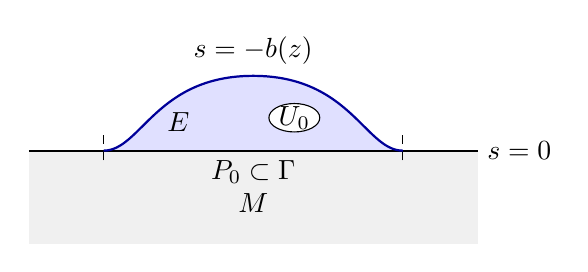
\begin{tikzpicture}[scale=0.95]
 \fill[gray!12] (-3,-1.25) rectangle (3,0);
 \fill[blue!12] (-2,0) .. controls (-1.5,0) and (-1.3,1.0) .. (0,1.0)
                 .. controls (1.3,1.0) and (1.5,0) .. (2,0) -- cycle;
 \draw[thick] (-3,0)--(3,0);
 \draw[thick,blue!60!black] (-2,0)
                 .. controls (-1.5,0) and (-1.3,1.0) .. (0,1.0)
                 .. controls (1.3,1.0) and (1.5,0) .. (2,0);
 \draw[dashed] (-2,-0.13)--(-2,0.23);
 \draw[dashed] (2,-0.13)--(2,0.23);
 \node at (0,-0.7) {$M$};
 \node at (-1,0.38) {$E$};
 \draw[fill=white] (0.55,0.44) ellipse (0.34 and 0.19);
 \node at (0.55,0.44) {$U_0$};
 \node[above] at (0,1.02) {$s=-b(z)$};
 \node[below] at (0,0) {$P_0\subset\Gamma$};
 \node[right] at (3,0) {$s=0$};
\end{tikzpicture}
\caption{A local schematic cross-section of the common exterior cap.
The boundary moves only over a compact subset of the measured patch.
The oval is a nonempty open source set $U_0$ with closure inside $E$.
The proof uses the smooth graph, including its flat bump edges.}
\label{data:cap-figure}
\end{figure}

\subsection{Harmonic tests from sources in the cap}

For $f\in C_c^\infty(U_0)$, let $u_f^j$ be the zero-Dirichlet solution
of $L_{g_j}u_f^j=f$ on $M_j^e$. Define its evaluation at a point by
\begin{equation}\label{data:evaluations}
 I_j(p)(f)=u_f^j(p).
\end{equation}
Equality of evaluations means equality for every such source $f$.
Proposition~\ref{data:cap} gives $I_1=I_2$ on $E$. The functions
$u_f^j$ are harmonic away from $\overline{U_0}$; we only use their
harmonic jets there.

This use of harmonic evaluations follows the Poisson and source
embedding approaches of \citet[Sections~2 and~6.1]{LLS20}.
The restricted-source approximation and separation results appear in
\citep[Appendix~A, Propositions~A.6--A.7]{LLS20}.
Unique continuation forces the inverse of an annihilating point
distribution to have point support, and differential order then
determines that distribution. We give the full argument for the
required second jets and positive densities.

\begin{lemma}[Separation and finite harmonic jets]\label{data:jet-family}
Let $(N,g)$ be a compact connected smooth manifold with nonempty
boundary and dimension $n\ge2$. Let $U\Subset N^\circ$ be
nonempty and open, and let $R=L_{g,D}^{-1}$. Then:
\begin{enumerate}[label=\textup{(\roman*)}]
 \item The functionals $I(p):f\mapsto Rf(p)$,
       $f\in C_c^\infty(U)$, separate distinct interior points.
       They are nonzero in the interior and zero on the boundary.
       For each fixed $f$, they depend continuously on $p\in N$.
 \item If $p\in N^\circ\setminus\overline U$, the second jets of
       $Rf$ at $p$ fill exactly the hyperplane defined by
       $L_g u(p)=0$. In particular they provide harmonic coordinates
       near $p$ and any finite spanning family of harmonic Hessians
       in those coordinates.
\end{enumerate}
\end{lemma}

\begin{proof}
Continuity and the zero boundary values follow from smooth Dirichlet
regularity. Nonvanishing follows by the same point-support argument
used below: if $I(p)=0$, then $w=R\delta_p$ vanishes on $U$ and
$L_gw=\delta_p$. Elliptic regularity and unique continuation on
the punctured connected interior force $w$ to be point-supported.
A nonzero point-supported distribution has elliptic image of order
at least two, and cannot have the order-zero image $\delta_p$.
If $p\in U$, the equation on $U$ already contradicts $w|_U=0$.

We prove the jet assertion by finite-dimensional duality. Let $T$
be a linear functional on second jets at $p$ annihilating all
$Rf$, represented as a distribution of order at most two supported
at $p$. Define $w=RT$ by transposition with the metric density.
The Dirichlet inverse is self-adjoint, so
\[
 \langle w,f\rangle=\langle T,Rf\rangle=0,
           \qquad f\in C_c^\infty(U).
\]
Thus $w=0$ on $U$ and $L_gw=T$. Away from $p$ it is smooth and
harmonic by elliptic regularity. The punctured interior is connected:
a path meeting $p$ can be diverted in a small punctured coordinate
ball, whose spheres are connected in dimension at least two.
Unique continuation consequently gives $\supp w\subset\{p\}$.

A distribution supported at one point is a finite sum
\[
 w=\sum_{|\alpha|\le k}c_\alpha\partial^\alpha\delta_p.
\]
If $w\ne0$ and $k$ is its highest derivative order, then $L_gw$
has exact order $k+2$. Indeed its highest coefficient polynomial
is the product of the nonzero degree-$k$ coefficient polynomial
and the nonzero elliptic quadratic principal symbol. Such a product
cannot vanish. Since $T$ has order at most two, $w=c\delta_p$.
Hence the annihilator consists precisely of multiples of
$u\mapsto L_gu(p)$. That functional does annihilate the source
solutions because $p\notin\overline U$. Finite-dimensional duality
proves that their jet range is the whole stated hyperplane.

To prove separation, suppose $I(p)=I(q)$ for distinct interior
points. Apply the same transposition argument to
$T=\delta_p-\delta_q$. The solution $RT$ vanishes on $U$,
and UCP on the connected interior with these two points removed
shows that it is supported at those points. The argument still
applies if a point lies in $U$, since the initial vanishing on $U$
is distributional. At each support point a nonzero point-supported
distribution has an elliptic image of order at least two.
It cannot have the order-zero image $\delta_p-\delta_q$.
This contradiction proves separation.

Finally the equation constraint allows arbitrary first derivatives,
by adjusting the Hessian. Choose $n$ source solutions with independent
differentials; their tuple is a harmonic coordinate chart. In this
chart the first-order coefficients of $\Delta_g$ vanish, so the
ordinary coordinate Hessians have precisely the constraint
$g^{ab}\partial_{ab}u=0$. The jet conclusion supplies a basis for
that hyperplane, with zero first derivatives if desired. A chosen
finite basis remains spanning, with a positive Gram bound, after
shrinking the chart.
\end{proof}

\begin{remark}\label{data:local-pairs}
At any point outside $\overline{U_0}$ we may use finitely many
pairs $(u_f^1,u_f^2)$ to supply the harmonic coordinates and Hessians
in the local argument. Once chosen, these functions remain fixed
while the spatial scales shrink. The constant pair $(1,1)$ is
adjoined separately; it is not a zero-boundary source solution.
All these statements are scalar and use positive densities, so
they retain nonorientable manifolds and arbitrary boundary components.
\end{remark}

% Derived from OpenAI, September 24, 2026, Apache-2.0.
% Modified October 12, 2026: explicit inputs, attribution, and full-data conclusion.
\section{Local continuation and product solutions}
\label{cross:section}

\subsection{The local metric extension theorem}

The common cap gives an initial isometry. To enlarge it, the global
argument will use source-generated harmonic coordinates to identify
neighborhoods of two interior points. In these coordinates we must
continue equality of the metrics across a point where equality is
already known on one side. The following theorem is the local input.

\begin{theorem}[Local metric extension]\label{local:extension}
Let $n\geq3$.  Let $(N_1,g_1)$ and $(N_2,g_2)$ be smooth compact
connected Riemannian manifolds with nonempty smooth boundary, with
Dirichlet Green functions $G_1,G_2$.  Identify two interior harmonic
coordinate neighborhoods with one neighborhood $\Omega\subset
\mathbb R^n$ of $0$.  Suppose an open $W\subset\Omega$ contains, near
$0$, one side of a smooth hypersurface through $0$, and suppose
\[
 g_1=g_2\text{ on }W,\qquad
 G_1(x,y)=G_2(x,y)\quad(x,y\in W,\ x\ne y).
\]
Suppose there are finitely many smooth pairs $u_j^a$ harmonic for
$g_j$ on $\Omega$, agreeing on $W$, whose first-side coordinate
Hessians at $0$ span
\[
 \{H\in\operatorname{Sym}^2(\mathbb R^n):g_1^{ij}(0)H_{ij}=0\}.
\]
Then the two coordinate metrics agree on a neighborhood of $0$.
\end{theorem}

We prove this theorem in Section~\ref{sec:bootstrap}. Its proof first
constructs a mixed Green kernel that is harmonic for the first metric in
$x$ and for the second metric in $y$: initially it is $G_1(x,y)$
when $y\in W$ and $G_2(x,y)$ when $x\in W$. For each prescribed
compact region at positive separation from $x=y$, a sufficiently small
spatial dilation allows the continuation constructed in this section to
reach that region. Section~\ref{sec:balls} then continues it to a family
of small spheres centered at $y$, under a temporary bound that controls
a normalized difference of the inverse metrics, together with finitely
many derivatives, by the current radius. Its flux transfers
first-metric harmonic functions to second-metric harmonic functions.
In particular, the resulting functional sends $u_1^a$ to $u_2^a$ and
reproduces the constant and coordinate functions.

The remaining task is uniform control as the spheres shrink.
Section~\ref{sec:angular} estimates the density representing the flux
functional. Under the same temporary metric bound, this estimate and exact
reproduction of affine functions give an $L^2$ bound for each paired
harmonic difference divided by the squared radius.
Section~\ref{sec:bootstrap} combines it with the spanning harmonic
Hessians to improve the temporary bound strictly. This improvement
allows the shrinking parameter to tend to zero with the spatial dilation
fixed, forcing the two metrics to be conformal near the contact point.
The common harmonic coordinates remove the remaining conformal factor. The geometric
continuation in this section provides existence away from the diagonal;
its estimates need not remain bounded as the separation tends to zero.

\subsection{Product solutions and extension from a cross}

We begin with a statement for general scalar elliptic operators. Let
$L_i$ be a smooth scalar second-order elliptic operator in a coordinate
domain, with real positive definite principal matrix $g_i^{-1}$.
Lower-order terms are allowed. A \emph{product solution} is a function
$F(x,y)$ satisfying
\[
 L_1^xF=0,\qquad L_2^yF=0.
\]
Such a function has ordinary unique continuation, since $L_1^x+L_2^y$
is elliptic on the product. We shall construct extensions explicitly;
unique continuation will identify extensions already constructed.

The starting data consist of two compatible product sets, with one
variable restricted to a smaller observed set in each piece. A common
basis for a solution space and its restriction to the smaller set will
construct the extension. We give the variable-coefficient singular-function argument,
including its quantitative dependence.

\begin{lemma}[Extension from a cross]\label{cross:series}
Let $D_i$ be bounded connected coordinate domains and
$S_i\Subset D_i$ nonempty open sets.  Suppose a product solution $F$ is
given consistently on
\[
 (D_1\times S_2)\cup(S_1\times D_2),
\]
with the sum of its two $L^2$ norms at most $M$.
Let $O_i\Subset D_i$ be open sets such that every $L_i$-solution $w$
on $D_i$ satisfies
\begin{equation}\label{cross:interpolation-input}
 \|w\|_{L^2(O_i)}
 \le C\|w\|_{L^2(S_i)}^{\gamma_i}
          \|w\|_{L^2(D_i)}^{1-\gamma_i},
 \qquad 0<\gamma_i<1,\qquad \gamma_1+\gamma_2>1.
\end{equation}
Then $F$ extends as a product solution to $O_1\times O_2$, agreeing
with both given pieces on their intersections.  On every compact
subset of this product its $C^m$ norm is at most $C_mM$.
The constants are uniform when the geometric margins, ellipticity,
coefficient bounds, interpolation constants and positive exponent
margin are uniform.  Each specified output order uses only finitely
many coefficient bounds.
\end{lemma}

\begin{proof}
Let $\mathcal H_1(D_1)$ be the closed subspace of $L^2(D_1)$ consisting
of distributional $L_1$-solutions. Restriction
$R:\mathcal H_1(D_1)\to L^2(S_1)$ is compact and injective. To prove
compactness, multiply each solution by a cutoff equal to one near
$\overline{S_1}$ and compactly supported in $D_1$. Interior estimates
bound its $H^q$ norm by its $L^2(D_1)$ norm. Fourier truncation in a
containing cube gives a finite-rank approximation to $R$ of rank
$O(A^n)$ and operator error $O(A^{-q})$. Hence $R$ is compact;
injectivity follows by unique continuation. The spectral theorem
for $R^*R$ gives an orthonormal basis $(w_j)$ of
$\mathcal H_1(D_1)$ such that
\begin{equation}\label{cross:singular-values}
 (w_i,w_j)_{L^2(S_1)}=\mu_j^2\delta_{ij},
 \qquad 0<\mu_j\le1.
\end{equation}
For every $N$,
\begin{equation}\label{cross:singular-decay}
 \mu_j\le C_N(1+j)^{-N}.
\end{equation}
Indeed let $K$ be the rank-$r$ approximation just constructed. Its
restriction to the span of the first $r+1$ eigenvectors has a unit
kernel vector $v$, for which
$\|(R-K)v\|=\|Rv\|\ge\mu_{r+1}$. Thus
$\mu_{r+1}\le\|R-K\|$. The Fourier bound with arbitrary integer $q$
yields $\mu_j\le C_qj^{-q/n}$ and proves the assertion, with the
stated uniformity. If the space is finite dimensional, the corresponding
finite sum needs no decay argument.

For $y\in S_2$ expand $F(\cdot,y)$ on $D_1$:
\[
 F(x,y)=\sum_j w_j(x)b_j(y),\qquad
 \|b_j\|_{L^2(S_2)}\le M.
\]
Equation~\eqref{cross:singular-values} continues these coefficients to
$D_2$ by the formula
\begin{equation}\label{cross:coefficient-extension}
 b_j(y)=\mu_j^{-2}\int_{S_1}F(x,y)\overline{w_j(x)}\,\dd x,
 \qquad \|b_j\|_{L^2(D_2)}\le M\mu_j^{-1}.
\end{equation}
The integral solves $L_2b_j=0$ and agrees with the original coefficient
on $S_2$.  Applying \eqref{cross:interpolation-input} gives
\[
 \|w_j\|_{L^2(O_1)}\le C\mu_j^{\gamma_1},\qquad
 \|b_j\|_{L^2(O_2)}\le CM\mu_j^{\gamma_2-1}.
\]
Consequently the series converges absolutely in $L^2(O_1\times O_2)$:
its summands are bounded by $CM\mu_j^{\gamma_1+\gamma_2-1}$.
Choose $N$ in \eqref{cross:singular-decay} so that
$N(\gamma_1+\gamma_2-1)>1$.  The limit solves both equations
in distributions.  Interior estimates for their elliptic sum give
the asserted smoothness and bounds on smaller sets.

We verify agreement with the second given piece; no assertion that
an arbitrary local solution extends to $D_1$ is needed.  Let $z$ be
orthogonal to the closure of $R\mathcal H_1(D_1)$ in $L^2(S_1)$.
The function
\[
 y\longmapsto\int_{S_1}F(x,y)\overline{z(x)}\,\dd x
\]
solves the second equation and vanishes on $S_2$, so it vanishes on
connected $D_2$.  Thus each second-piece slice belongs to that closed
range.  Its expansion in the orthonormal basis $w_j/\mu_j$ is complete,
and its coefficients are $\mu_jb_j(y)$ by
\eqref{cross:coefficient-extension}.  It follows that the series is
$F$ on $S_1\times O_2$; the series converges there also by the positive
exponent $\gamma_2$.  On $O_1\times S_2$ it is the original expansion,
with positive exponent $\gamma_1$.  This proves both agreements.
Only upper bounds for the singular values were used, so uniformity
does not require continuous choices of singular bases or positive
lower bounds for their singular values.
\end{proof}

Figure~\ref{cross:figure} summarizes the sets and the two estimates in
Lemma~\ref{cross:series}.
\begin{figure}[htbp]
 \centering
 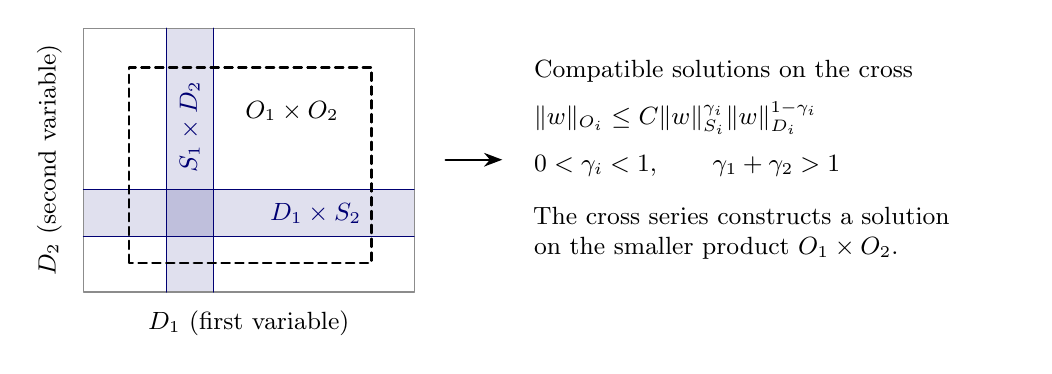
\begin{tikzpicture}[x=1cm,y=1cm,font=\small,>=Stealth,
  line cap=round,line join=round]
  \colorlet{crossink}{blue!45!black}
  \fill[crossink!12] (0,0.70) rectangle (4.2,1.30);
  \fill[crossink!12] (1.05,0) rectangle (1.65,3.35);
  \fill[crossink!25] (1.05,0.70) rectangle (1.65,1.30);
  \draw[black!45] (0,0) rectangle (4.2,3.35);
  \draw[crossink,thin] (0,0.70)--(4.2,0.70)
    (0,1.30)--(4.2,1.30) (1.05,0)--(1.05,3.35)
    (1.65,0)--(1.65,3.35);
  \draw[densely dashed,thick] (0.58,0.37) rectangle (3.66,2.85);
  \node[fill=white,inner sep=3pt] at (2.65,2.30) {$O_1\times O_2$};
  \node[text=crossink] at (2.95,1.00) {$D_1\times S_2$};
  \node[text=crossink,rotate=90] at (1.35,2.10) {$S_1\times D_2$};
  \node[anchor=north] at (2.10,-0.12) {$D_1$ (first variable)};
  \node[rotate=90,anchor=south] at (-0.15,1.68) {$D_2$ (second variable)};
  \draw[->,thick] (4.60,1.68)--(5.32,1.68);
  \node[anchor=west,align=left,text width=6.10cm] at (5.60,1.68) {
    Compatible solutions on the cross\\[6pt]
    $\displaystyle
       \|w\|_{O_i}\leq C\|w\|_{S_i}^{\gamma_i}
                              \|w\|_{D_i}^{1-\gamma_i}$\\[6pt]
    $\displaystyle 0<\gamma_i<1,\qquad \gamma_1+\gamma_2>1$\\[8pt]
    The cross series constructs a solution\\
    on the smaller product $O_1\times O_2$.
  };
\end{tikzpicture}

 \caption{Compatible product solutions are given on the shaded cross.
 The $L^2$ interpolation estimates for single-variable solutions,
 with $\gamma_1+\gamma_2>1$, make the
 singular-function series converge on $O_1\times O_2$.
 The drawing is schematic: each factor is a multidimensional domain,
 and containment of $S_i$ in $O_i$ is not required.}
 \label{cross:figure}
\end{figure}

\subsection{A geometric criterion for local extension}

We next build the interpolation estimates needed in
Lemma~\ref{cross:series}.  For a metric $g$, call a smooth real function
$\theta$ a \emph{strict weight} at a point where $\dd\theta\ne0$ if
\begin{equation}\label{cross:strict-weight}
 \operatorname{Hess}_g\theta(e,e)
  +\operatorname{Hess}_g\theta(v,v)>0
 \quad\text{for all }v\perp e,\ |v|_g=1,
 \qquad e=\frac{\nabla^g\theta}{|\nabla^g\theta|_g}.
\end{equation}
The strict scalar Carleman estimate gives, after shrinking the
coordinate neighborhood,
\begin{equation}\label{cross:carleman}
 \tau^3\|e^{\tau\theta}w\|_{L^2}^2
 +\tau\|\nabla(e^{\tau\theta}w)\|_{L^2}^2
 \le C\|e^{\tau\theta}Lw\|_{L^2}^2,
 \qquad \tau\ge\tau_0,
\end{equation}
for compactly supported $w$.
This is the elliptic strict-weight estimate of the classical
Carleman theory; see
\citet[Definition~8.3 and Theorem~9(a)]{KochTataru2005}.
Here the hypotheses can also be checked directly.  For $L=-\Delta_g$,
write $v=e^{\tau\theta}w$ and
\[
 e^{\tau\theta}Le^{-\tau\theta}=A_\tau+B_\tau,\qquad
 A_\tau=-\Delta_g-\tau^2|\dd\theta|_g^2,\quad
 B_\tau=\tau(2\nabla^g\theta\cdot\nabla+\Delta_g\theta).
\]
Here $A_\tau$ is self-adjoint and $B_\tau$ is skew-adjoint for
metric volume.  Integration by parts gives
\begin{align*}
 \|(A_\tau+B_\tau)v\|^2
 &=\|A_\tau v\|^2+\|B_\tau v\|^2
       +([A_\tau,B_\tau]v,v),\\
 ([A_\tau,B_\tau]v,v)
 &=4\tau\int\operatorname{Hess}_g\theta(\nabla v,\nabla\overline v)
   +4\tau^3\int\operatorname{Hess}_g\theta
                 (\nabla\theta,\nabla\theta)|v|^2
   -\tau\int(\Delta_g^2\theta)|v|^2.
\end{align*}
Choose a real constant $m$ strictly between the negative of the least
unit tangential Hessian value and the unit normal Hessian value.
After shrinking the patch, these inequalities have a positive margin.
Add $4m\tau(A_\tau v,v)$ to the commutator form.  Its gradient
coefficient becomes $4\tau(\operatorname{Hess}_g\theta+mg)$,
and its leading zero-order coefficient is
\[
 4\tau^3|\dd\theta|_g^2
       \big(\operatorname{Hess}_g\theta(e,e)-m\big)>c\tau^3.
\]
The tangential gradient form is positive.  Its mixed and possibly
negative normal terms cost at most
$C\tau\|\nabla_e v\|^2$, and
\[
 \|\nabla_e v\|^2
 \le C\tau^{-2}\|B_\tau v\|^2+C\|v\|^2.
\]
Finally
$|4m\tau(A_\tau v,v)|\le\tfrac12\|A_\tau v\|^2+
C\tau^2\|v\|^2$.
For large $\tau$, the squared parts absorb the normal derivative
cost and the positive zero-order term absorbs the remaining errors.
This yields \eqref{cross:carleman}.  Smooth first- and zero-order terms
in $L$ cost only $C(\|\nabla v\|^2+\tau^2\|v\|^2)$ and are absorbed
in the same way.  The proof gives uniform constants on fixed compact
sets of strict weights and bounded coefficients.

The existence criterion is a condition on a hypersurface in the
product.  Hessians in the following statement use the product
connection of $g_1$ and $g_2$.

\begin{proposition}[Product extension criterion]\label{cross:criterion}
Let $\rho$ be smooth near $z_0=(x_0,y_0)$, with $\rho(z_0)=0$ and
$\dd_x\rho,\dd_y\rho\ne0$.  Put
\[
 a_i=\frac{\nabla_i\rho}{|\nabla_i\rho|^2},\qquad H=\operatorname{Hess}\rho.
\]
Suppose that at $z_0$
\begin{equation}\label{cross:hessian-test}
 H((a_1,-a_2),(a_1,-a_2))
 +H((v_1,v_2),(v_1,v_2))>0
 \quad
 \left(v_i\perp a_i,\ |v_i|=|a_i|\right).
\end{equation}
Every product solution given on $\{\rho>0\}$ near $z_0$ extends to
a neighborhood of $z_0$, agreeing on a smaller part of that side.
In fact, the construction uses only two compact product sets in
$\{\rho>\epsilon\}$ for some $\epsilon>0$.
The neighborhoods and estimates on smaller neighborhoods are uniform
under small smooth perturbations preserving the strict hypotheses,
provided the data on those compact sets are bounded.
\end{proposition}

\begin{proof}
We first split the product Hessian condition into a strict weight in
each factor. Their sum will lie below a defining function for the given
side, with a quadratic gap. That gap places two intersecting product
sets in the given side; the weights then yield interpolation exponents
greater than one half, allowing Lemma~\ref{cross:series} to apply.

\paragraph{Splitting the weight between the factors.}
We seek symmetric forms $P_i$ satisfying
\[
 P_i(a_i,a_i)+P_i(v_i,v_i)>0,
 \qquad H+K\,\dd\rho^{\otimes2}>P_1\oplus P_2
\]
for some $K>0$, with the vectors $v_i$ as in
\eqref{cross:hessian-test}. After division by $|a_i|^2$, the first
inequality is the strict-weight condition for a function with gradient
$\nabla_i\rho$ and Hessian $P_i$. The second inequality will give the
quadratic gap. To obtain these forms by convex separation, the dual
tests are positive semidefinite forms $D$ whose diagonal blocks are
\[
 d_i a_i^{\otimes2}+S_i,\qquad
 d_i\ge0,\quad S_i\ge0\text{ on }a_i^\perp,
 \quad \tr S_i=d_i|a_i|^2.
\]
Here is the finite-dimensional separation being used. If $C$ is an
open convex cone and $H\notin C$, fix $c_0\in C$ and put
$H_e=H-ec_0$. Then $H_e\notin\overline C$, since
$\overline C+C\subset C$. Let $q_e$ be the nearest point of
$\overline C$ to $H_e$, supplied by the Hilbert projection theorem.
The projection inequality, tested also at $0$ and $2q_e$, shows that
$D_e=(q_e-H_e)/|q_e-H_e|$ satisfies $D_e:C\ge0$ and
$D_e:H_e<0$. A convergent subsequence as $e\downarrow0$ gives
$|D|=1$, $D:C\ge0$, and $D:H\le0$. Apply this to the cone of positive
definite forms plus the allowed $P_1\oplus P_2$. The individual dual
cones consist exactly of the displayed diagonal blocks: diagonalizing
$S_i$ expresses such a block as a positive sum of
$a_i^{\otimes2}+v_i^{\otimes2}$; separation from this closed cone,
followed by a small positive-definite perturbation of the separator,
proves the converse. This proves the stated dual tests without an
additional convex representation theorem.
Normalize $\tr D=1$.  To obtain a suitable $K$, it suffices by
compactness to prove $H:D>0$ on tests with $D\,\dd\rho=0$.

Represent such a $D$ as a covariance matrix.  The normal components
measured by the two partial covectors are opposite.  The diagonal-block
condition makes each normal component uncorrelated with its own
tangential component, hence with both tangential components.
Their variances coincide, giving $d_1=d_2=d>0$ and
\[
 D=d(a_1,-a_2)^{\otimes2}+D_\perp,
 \qquad \tr(D_\perp)_{ii}=d|a_i|^2.
\]
The case $d=0$ would force $D=0$. Among nonnegative tangential forms
with the two fixed traces, minimize the linear functional $H:D_\perp$
on their compact set, and choose a minimizer of least rank. If its rank
is $r\ge2$, a nonzero symmetric perturbation supported on its image
preserves both traces, since $r(r+1)/2>2$. Both small signs preserve
positivity, so minimality forces the objective to be constant in this
direction. Continuing to an endpoint of positivity lowers the rank,
a contradiction. The perturbation has trace zero and is nonzero, so
has both signs and such an endpoint is finite. The minimizer therefore
has rank one. Its two fixed traces give exactly the rank-one tests
in \eqref{cross:hessian-test}, multiplied by $d$; their strict positivity
proves $H:D>0$ for every test under consideration. Compactness of the
normalized tests then supplies $K$, as required. Explicitly, if no $K$
worked, separators with trace one for $H+K\,\dd\rho^{\otimes2}$,
as $K\to\infty$, would have a limit with $D\,\dd\rho=0$ and
$H:D\le0$, contradicting the positivity just proved.

Prescribe gradients $\dd_i\rho$ and Hessians $P_i$ for smooth functions
$\theta_i$ vanishing at the respective points.  In small coordinates
centered there, Taylor expansion gives
\begin{equation}\label{cross:quadratic-gap}
 \theta_1(x)+\theta_2(y)
 \le \widetilde\rho(x,y)-c(|x|^2+|y|^2),
 \qquad \widetilde\rho=\rho+K\rho^2/2,
\end{equation}
with $c>0$.  Each $\theta_i$ satisfies
\eqref{cross:strict-weight}.  The positive side of $\widetilde\rho$
is the positive side of $\rho$ in this neighborhood.

\paragraph{Placing the cross and obtaining interpolation.}
Use coordinates $(s_i,z_i)$ with $s_i=\theta_i$. Fix a small
$\kappa>0$ so that $\phi(s_i)=s_i-\kappa s_i^2$ remains a strict weight.
Choose successively a small lateral radius $R$, a height
$l\ll cR^2$, and $e\ll\kappa l^2$.  Take
\[
 D_i=\{-l<s_i<l+4e,\ |z_i|<R\}.
\]
Use a cutoff equal to one on the inner lateral half and for
$-l+3e<s_i<l+2e$, supported in the cylinder and in
$-l+2e<s_i<l+3e$.
Let $S_i\Subset D_i$ include neighborhoods of its top and lateral
derivative supports, where respectively
\[
 s_i>l+e/2\quad\text{or}\quad |z_i|>R/3,
\]
and an inner top slice near $s_i=l+5e/4$.
The two closed product sets $\overline{D_1\times S_2}$ and
$\overline{S_1\times D_2}$ lie strictly in the given side.
For a top slice, the sum of the two $s$ coordinates is positive.
For a lateral slice, it is greater than $-2l$, which is dominated
by the quadratic gap in \eqref{cross:quadratic-gap}.
Making the sets slightly smaller if necessary gives a common
$\epsilon>0$ with $\rho>\epsilon$ on their closures.

For an $L_i$-solution normalized by $\|w\|_{L^2(D_i)}=1$, apply
\eqref{cross:carleman} to this cutoff times $w$.  Interior estimates
bound the bottom derivative terms using the large norm and the weight
$\phi(-l+3e)$.  The remaining derivative terms use
$\|w\|_{L^2(S_i)}$ and a weight at most $\phi(l+3e)$.
On a smaller inner cylinder beginning at $s_i=-e$, the weight is at
least $\phi(-e)$.  Balancing the two exponentials yields
\eqref{cross:interpolation-input} with
\begin{equation}\label{cross:exponent}
 \gamma_i=
 \frac{\phi(-e)-\phi(-l+3e)}{
       \phi(l+3e)-\phi(-l+3e)}>\frac12.
\end{equation}
Indeed at $e=0$ the quotient is $1/2+\kappa l/2$.
Values of the balancing parameter below $\tau_0$ are covered by
increasing the constant.  The output cylinder may be chosen to include
a connected tube from the origin to the indicated top slice.

\paragraph{Constructing and identifying the extension.}
Lemma~\ref{cross:series} now gives a product solution on a neighborhood
of $z_0$. It agrees with the old solution there on the positive side:
from a sufficiently near positive-side point, increase $s_2$ into
the top slice.  Since $\partial_{s_2}\rho>0$ locally, the segment stays
on that side and in the larger constructed cylinder.  Agreement on
the slice and unique continuation along a neighborhood of the segment
prove agreement at the original point.
All choices have strict margins.  Keeping their finitely many compact
sets and shrinking their output neighborhoods once proves the stated
perturbation uniformity by \eqref{cross:carleman},
Lemma~\ref{cross:series} and interior elliptic estimates.
\end{proof}

\subsection{Gluing along a compact family of surfaces}

Proposition~\ref{cross:criterion} provides a germ across one surface
point.  The following formulation records the geometry needed to
combine these germs.  In particular, agreement is proved on specified
overlap components, rather than inferred from the existence of a cover.

\begin{lemma}[Propagation through a compact cylinder]
\label{cross:propagation}
Suppose a region in a product patch has smooth coordinates $(z,a)$
near $B\times[a_-,a_+]$, where $B$ is a compact base, possibly with
boundary or corners.  A product solution is given on a neighborhood
of the top and lateral boundary and on an open set $\mathcal S$.
Assume that $\mathcal S$ is upward closed in $a$ at fixed $z$ and
contains these boundary neighborhoods.  If every level $a=\text{constant}$
satisfies Proposition~\ref{cross:criterion} outside $\mathcal S$, with
the positive side pointing toward increasing $a$, the solution extends
to a neighborhood of the cylinder, agreeing on $\mathcal S$.
For fixed coordinates, compact sets and strict reference inequalities,
the extension has uniform compact-subset bounds under small smooth
perturbations, in terms of bounds on finitely many compact subsets of
the initially given region.
\end{lemma}

\begin{proof}
Starting from the top, let $a_*$ be the infimum of levels down to which
an extension agreeing with the seed has been obtained.  In the uniform
version include uniform bounds in this property.  At a non-seed point
of $B\times\{a_*\}$, Proposition~\ref{cross:criterion} uses compact
data strictly above that level.  Take a finite cover of the level by
such output neighborhoods and seed neighborhoods.  Their data are
contained above $a_*+\eta$ for one $\eta>0$, so an already reached
level supplies them with the needed bounds.

Shrink the outputs in $(z,a)$ coordinates to boxes
$B_i\times(a_*-d_i,a_*+d_i)$.
Every connected component of an overlap contains vertical segments
to a common height greater than $a_*$.  Both germs equal the preceding
extension there.  Unique continuation for $L_1^x+L_2^y$ makes them
identical on that overlap component.  The same argument gives agreement
with $\mathcal S$, because a vertical segment moving upward from a
seed point stays in the seed.  Boundary neighborhoods use the given
solution.  A finite subcover has a positive minimum output width and
therefore passes the putative last level, or includes the endpoint
$a_-$.  This proves continuation on the whole cylinder.
The same finite constructions retain all strict margins under small
perturbations.  Their Carleman, series and interior estimates prove
the uniform assertion.  Data bounded up to a limiting surface are
never required: each local construction uses compact sets strictly
above it.
\end{proof}

\subsection{Initialization at a fixed distance from the diagonal}

We apply the criterion to a mixed Green kernel.  Let $g_1,g_2$ be smooth
metrics in coordinate patches centered at $0$, obtained from interior
patches of compact Dirichlet manifolds.  Suppose they agree on an open
set $W$ containing the lower side of a smooth hypersurface through $0$.
After a linear coordinate change, assume
\[
 g_1(0)=g_2(0)=I,\qquad
 \{x_n<q(x')\}\subset W\text{ near }0,\qquad
 q(0)=0,\quad \dd q(0)=0,
\]
for a smooth function $q$.  No regularity of the rest of $\partial W$
is assumed.
Let $G_j$ be the Dirichlet Green kernels, normalized with metric volume,
and suppose $G_1=G_2$ on $W\times W$.
For a small dilation parameter $\lambda>0$, put
\begin{equation}\label{cross:dilation}
 g_{j,\lambda}(z)=g_j(\lambda z),\qquad
 G_{j,\lambda}(x,y)=\lambda^{n-2}G_j(\lambda x,\lambda y),
 \qquad W_\lambda=\lambda^{-1}W.
\end{equation}
On each fixed bounded patch the metrics tend smoothly to the Euclidean
metric, and $W_\lambda$ contains every fixed compact subset of
$\{z_n<0\}$ for sufficiently small $\lambda$.
Initially define, off the diagonal,
\begin{equation}\label{cross:mixed-data}
 \mathcal G_\lambda(x,y)=
 \begin{cases}
 G_{1,\lambda}(x,y),&y\in W_\lambda,\\
 G_{2,\lambda}(x,y),&x\in W_\lambda.
 \end{cases}
\end{equation}
The pieces fit and solve the first equation in $x$ and the second in $y$.

\begin{proposition}[Fixed-separation initialization]\label{cross:initial}
In this setting, let $n\ge3$ and fix $B>0$, $d>0$ and $\eta>0$.
For all sufficiently small $\lambda$, the data
\eqref{cross:mixed-data} have a product-solution continuation to a
neighborhood of
\[
 \{(x,y):|x|,|y|\le B,\ |x-y|\ge d\}.
\]
Every fixed $C^m$ norm on a smaller neighborhood is bounded uniformly
in $\lambda$.  The continuation agrees with $G_{1,\lambda}$ where
$y_n<-\eta$ and with $G_{2,\lambda}$ where $x_n<-\eta$, on the
corresponding overlaps.  The smallness threshold for $\lambda$ and
the constants may depend on $B,d,\eta,m$.
\end{proposition}

\begin{proof}
We first cross the limiting plane, then deform variable-radius tubes
to reach the prescribed separations.  All the sets and positive
separation margins used in the two steps are fixed before choosing
$\lambda$.

\paragraph{Crossing the plane and obtaining a common seed.}
We first extend slightly across the plane in one variable while keeping
the other at a comparable positive separation. The first interpolation
exponent can be made close to one; this compensates for the fixed
positive exponent obtained by propagation in the separated second
variable.

Fix a point $x_0$ of height zero and a separation scale $s>0$.
In the second factor take
\[
 D_2=\{s/2<|y-x_0|<2s\}
\]
and an observed ball $S_2$ about $x_0-se_n$.
In the first take a ball of radius $3\tau_0s$ centered at
$x_0-\tau_0se_n$, with $\tau_0>0$ fixed small enough that the two
large domains are separated.  Its observed ball has radius
$(1-\alpha)\tau_0s$, with $\alpha>0$ to be chosen.
These observed balls lie strictly in the lower half-space.

There is a two-constants estimate from $S_2$ to a slightly enlarged
closed annulus $4s/5\le|y-x_0|\le6s/5$, with an exponent
$\gamma_2>0$ independent of $\alpha$.  Here is a direct way to obtain
it with room for perturbations.  On a Euclidean annulus the weight
$|z-z_*|^{-1}$ is strict: its radial Hessian is
$2|z-z_*|^{-3}$ and each tangential Hessian value is
$-|z-z_*|^{-3}$.  Radial cutoffs in
\eqref{cross:carleman}, followed by exponential balancing, propagate
smallness from an inner ball to an intermediate ball using the norm
on an outer ball.  A finite chain of overlapping balls with enlarged
balls inside $D_2$ connects $S_2$ to the target annulus.  The annulus
is connected since $n\ge3$.  Multiplying the finitely many positive
exponents gives the asserted $\gamma_2$.  The same weights and margins
work for sufficiently small perturbations of the Euclidean metric.

In the first factor use this radial argument centered at
$x_0-\tau_0se_n$.  Keep the outer cutoff a fixed distance beyond radius
$\tau_0s$, and put the inner cutoff just inside radius
$(1-\alpha)\tau_0s$.  Take a concentric target ball of radius
$(\tau_0+c)s$, with $c>0$ small; it contains the observed ball and
a ball of radius $cs$ about $x_0$.
As $\alpha$ and $c$ decrease, the target weight approaches the inner weight.
The interpolation exponent therefore tends to one.  Choose these
constants so that $\gamma_1+\gamma_2>1$.
Lemma~\ref{cross:series} extends the kernel to a small ball about
$x_0$ times the target annulus.  On these fixed separated sets the
rescaled Green kernels and their derivatives are uniformly bounded:
the local Green singularity is $O(|x-y|^{2-n})$, and interior elliptic
estimates give derivative bounds away from the pole.

The extensions agree with both lower pieces.  Agreement for $y\in S_2$
comes from the first expansion.  For fixed $x$ below a sufficiently
small negative height, continue in $y$ through the connected target
annulus to compare with $G_{2,\lambda}$.  For a second point below that
height, compare with $G_{1,\lambda}$ by continuation in the first
variable from its observed ball.  All comparisons remain separated.

The local extensions must next be compared on overlaps. Retain much
smaller first balls and narrower annuli for coverage, keeping the larger
products as comparison domains. The unused margins allow both variables
to move into the known lower region. Overlapping retained products have
scales comparable to $|x-y|$. For two products of the same orientation,
lower their near-plane variable into the known region; the path stays
inside both larger first balls.  For products of opposite orientations,
both variables lie in retained near-plane balls. On the fixed compact
range of locations and positive separation scales, choose the retained
products with strict ball and annular margins, then take $\eta_0>0$
much smaller than the smallest retained width. Lower both variables by
\[
 h=\max(x_n,y_n,0)+2\eta_0.
\]
By making the retained balls a sufficiently small fraction of the larger
balls, the path stays in both larger products: its displacement is
smaller than their ball and annular margins. Its endpoint has both
heights below $-\eta_0$,
where both germs are the original kernel.  Unique continuation along
a neighborhood of the path proves agreement.  Choose
$\eta_0\le\eta$ and then $\lambda$ small enough for this truncated
lower half-space to lie in $W_\lambda$ on all sets used.

Interchanging the two variables and covering gives, for some fixed
$c_0>0$, a single-valued continuation in
\begin{equation}\label{cross:coarse-region}
 \min(x_n,y_n)<c_0|x-y|,
\end{equation}
on every fixed compact range of bounded locations and positive
separations.  The estimates are uniform in $\lambda$ on that range.
For coverage near the plane, take $x_0=(x',0)$ and
$s=|y-x_0|$ when the first variable has the smaller nonnegative height;
then $x$ is in the retained first ball and $y$ in the retained annulus
if $c_0$ is small.  Points already below the plane are covered by the
same construction near it or by the given cross farther below it.
The preceding overlap argument makes these choices compatible.

\paragraph{Sweeping tubes inward from the common seed.}
The region \eqref{cross:coarse-region} is now the seed for the second
stage. At fixed center $y$ and direction $\omega$, we move $x$ along the
ray from $y$: large radii lie in the seed, and decreasing the radius
will reach the target pairs. Choose $M>B+3$ and introduce
\begin{equation}\label{cross:tubes}
 t=M+y_n+e_0|y'|^2,\qquad r_a(y)=a t^{1+\sigma},\qquad
 x=y+r_a(y)\omega,\quad |\omega|=1,
\end{equation}
where $\sigma,e_0>0$ will be small.  The base is
\[
 y_n\ge-B-1,\qquad t\le T_0,\qquad \omega\in\mathbb S^{n-1},
\]
and $a$ decreases through a fixed interval $[a_{\min},a_{\max}]$.
The term $e_0|y'|^2$ makes this base compact. The parameter $a$ decreases
while $(y,\omega)$ remains fixed, as required by the compact-cylinder
propagation lemma.
Take $a_{\min}$ small enough that the target separations exceed
$r_{a_{\min}}(y)$, and $a_{\max}$ large enough that its whole level
satisfies \eqref{cross:coarse-region}.  The bottom base boundary has
$y_n<0$.  Take $T_0$ so large that
$c_0a_{\min}T_0^\sigma>1$; its top boundary also satisfies
\eqref{cross:coarse-region}. Here the superlinear power $1+\sigma$
ensures that $r_a/t=a t^\sigma$ is large on this top face. Thus the
initial $a$-level and both base boundary faces are supplied by the seed.
This known region is upward closed in $a$: since
$\min(x_n,y_n)=y_n+r\min(\omega_n,0)$, its defining
inequality is $y_n<(c_0-\min(\omega_n,0))r$, whose radius coefficient
is positive.

It remains to check the strict extension criterion outside that region.
At the Euclidean metrics use
\[
 \rho=\tfrac12(|x-y|^2-r_a(y)^2),\qquad b=\nabla r_a.
\]
Away from $\omega+b=0$, multiply the vectors in
\eqref{cross:hessian-test} by the common positive factor $r_a$ and
write their real and imaginary parts as
\begin{equation}\label{cross:null-vectors}
 \begin{aligned}
 U_1&=\omega+iv,& |v|=1,\quad v\perp\omega,\\
 U_2&=\frac{\omega+b}{|\omega+b|^2}+iw,
 &w\perp(\omega+b),\quad |w|=|\omega+b|^{-1}.
 \end{aligned}
\end{equation}
The identity $\omega\cdot(U_1-U_2)=b\cdot U_2$ cancels the normal
part of the distance Hessian.  Consequently the test is
\begin{equation}\label{cross:tube-test}
 \big|\pi_{\omega^\perp}(U_1-U_2)\big|^2
 -(r_a\partial^2r_a)(U_2,\overline{U_2}).
\end{equation}
For bounded $b$, outside fixed small neighborhoods of
$b=-\omega$ and $b=-2\omega$, the first term is at least $c|b|^2$.
To see this, a zero forces the real part of $U_2$ to be parallel to
$\omega$, and equality of the projected imaginary lengths gives
$|\omega+b|=1$.  Thus $b=0$ or $b=-2\omega$.
Near $b=0$, the real projected difference controls
$|\pi_{\omega^\perp}b|$ to first order; also
\[
 |\pi_{\omega^\perp}w|
 =1-\omega\cdot b+O(|b|^2),
\]
so the imaginary projected difference controls $|\omega\cdot b|$
to first order.  This proves the quadratic lower bound near zero;
compactness proves it on the remaining range.

Outside \eqref{cross:coarse-region}, $y_n\ge c_0r_a$, so
$r_a/t\le1/c_0$ and
\[
 b=(1+\sigma)(r_a/t)\nabla t
\]
stays bounded.  When $\nabla t$ is close to $e_n$, the two excluded
neighborhoods already lie in \eqref{cross:coarse-region}.  Indeed,
\[
 \frac{x_n}{r_a}
 \le \frac{(1+\sigma)|\nabla t|}{|b|}+\omega_n,
\]
which is arbitrarily small near $b=-\omega$ and negative near
$b=-2\omega$ as $\sigma$ and the gradient error tend to zero.
On the complement $|U_2|$ is bounded and differentiation of
\eqref{cross:tubes} gives
\begin{equation}\label{cross:tube-error}
 r_a|\partial^2r_a|
 \le C(\sigma+T_0e_0)|b|^2.
\end{equation}
Choose the excluded-neighborhood sizes first in terms of $c_0$.
Use the positive lower bound on the remaining bounded $b$-range to
choose $\sigma$ small, then choose the $a$-interval and $T_0$ as above,
and finally $e_0>0$ so small that \eqref{cross:tube-error} is absorbed.
Choosing the transverse compactification last keeps its contribution
to the Hessian test small. These choices also make the gradient error small, since
$|\nabla t-e_n|\le2\sqrt{e_0T_0}$ on the base.
Thus \eqref{cross:tube-test} is strictly positive wherever continuation
is needed.  Both partial gradients are nonzero there.

All these sets are bounded and stay at separation at least
$a_{\min}(M-B-1)^{1+\sigma}>0$.  Smooth convergence of the metrics
therefore preserves the strict tests for sufficiently small $\lambda$.
Lemma~\ref{cross:propagation} continues the kernel through the cylinder,
with uniform estimates and agreement on the seed.  A target pair has
$a=|x-y|/t^{1+\sigma}\ge a_{\min}$; if $a>a_{\max}$ it is already in
the coarse region.  Hence every target pair is covered.

We also identify the extension with both pieces of the full cross
\eqref{cross:mixed-data}. Perform the construction with a larger bound
$B'>B$ and a smaller separation $0<d'<d$, chosen so that for every
$|y|\le B$ the domain
\[
 D_y=B(0,B')\setminus\overline{B(y,d')}
\]
is connected and contains a fixed lower open ball with $x_n<-\eta$.
Choose $B'$ large enough that every excluded closed ball lies strictly
inside $B(0,B')$ and is disjoint from that lower ball.
For fixed $y\in W_\lambda$ in the target range, the continuation
and $G_{1,\lambda}$ solve the same first-variable equation on $D_y$.
On the lower ball the continuation equals $G_{2,\lambda}$, which equals
$G_{1,\lambda}$ because both variables lie in $W_\lambda$.
Unique continuation on $D_y$ proves agreement on the required overlap.
Interchanging the variables proves agreement with the other piece.
Keeping slightly larger target bounds and a slightly smaller separation
before restricting to the prescribed range gives the claimed neighborhood
and its compact-subset estimates.
\end{proof}

The constants in Proposition~\ref{cross:initial} may deteriorate as
$d\downarrow0$.  Its role is to initialize a construction at finitely
many fixed positive scales.  Lemma~\ref{cross:propagation} will also
provide qualitative existence at each positive radius in a shrinking
family; the uniform estimate for that family is established below.

% Derived from OpenAI, September 24, 2026, Apache-2.0.
% Modified October 12, 2026: explicit inputs, attribution, and full-data conclusion.
\section{Continuation to shrinking spheres}\label{sec:balls}

We now apply the product continuation criterion near a point where an
isometry is already known on one side.  The purpose of this section is to
construct a family of functionals on harmonic functions, represented on
small spheres.  Their existence will follow from the geometry of the
spheres.  A uniform bound for the functionals, needed when the spheres
shrink, will follow from the estimate in the next section.

\subsection{The local data and their normalization}
\label{balls:setup}

Throughout Sections~\ref{sec:balls}--\ref{sec:bootstrap}, fix the
manifolds $(N_j,g_j)$, actual Dirichlet Green functions $G_j$, common
harmonic coordinate neighborhood $\Omega$, matching set $W$, and finite
harmonic pairs $(u_1^a,u_2^a)$ of Theorem~\ref{local:extension}.
Thus the coordinate metrics and paired functions agree on $W$, and the
Green kernels agree on $W\times W$ off the diagonal. The first-side
coordinate Hessians span the hyperplane annihilated by $g_1^{-1}(0)$. An interior ball in
$W$ tangent at $0$ supplies the one-sided hypersurface required by
that theorem. We construct the sphere functionals for these data.

A linear change of harmonic coordinates makes $g_1(0)=g_2(0)=I$ and
writes the separating hypersurface as a graph tangent to $x_n=0$, with
the known side below it.  For a spatial
dilation $\lambda>0$, write
\begin{equation}\label{balls:dilation}
 g_{j,\lambda}(x)=g_j(\lambda x),\qquad
 G_{j,\lambda}(x,y)=\lambda^{n-2}G_j(\lambda x,\lambda y).
\end{equation}
Dilate the harmonic pairs at the same time:
\[
 u_{j,\lambda}^a(x)=u_j^a(\lambda x).
\]
They remain harmonic for $g_{j,\lambda}$ and agree on the dilated known
set. The metrics and Green kernels in \eqref{balls:dilation} have the
corresponding normalization on the dilated neighborhoods. On each fixed
bounded coordinate set the metrics converge smoothly to $I$ as $\lambda\downarrow0$.  The dilated known set
contains every fixed compact set lying strictly below $x_n=0$, once
$\lambda$ is sufficiently small.

Use $x$ for the first variable and $y$ for the second.  The mixed kernel
$\mathcal G$ is initially $G_{1,\lambda}$ when $y$ is in the known set,
and $G_{2,\lambda}$ when $x$ is in that set.  These prescriptions agree on
their overlap and solve the first equation in $x$ and the second in $y$,
away from the diagonal.  Proposition~\ref{cross:initial} continues this
kernel to any specified compact region of fixed positive separation,
with smooth bounds uniform for small $\lambda$.  We shall use that result
only after all the positive separation ranges in question have been fixed.

The geometry of a moving sphere dictates the next choices. In the
strict extension test, the leading terms involving the gradient of its
radius cancel; strict concavity of the logarithmic radius supplies the
remaining positive term (see \eqref{balls:test-expression}). We therefore
choose a conformal reference metric for which a depth function is
strictly concave. Separately, a scalar normalization of the second
inverse metric will give the two inverse matrices the same trace
relative to the reference metric. The harmonic Hessians will determine
their remaining difference.

Fix the coordinate cylinder
\[
 Y=\{y=(y',y_n): |y'|\leq1,\ -1\leq y_n\leq1\},
 \qquad t_0(y)=y_n+|y'|^2.
\]
Take a sufficiently large fixed number $L$ and put
\begin{equation}\label{balls:normalization}
 \gamma=e^{-2Lt_0}g_{1,\lambda},\qquad
 Q=\frac{n\,g_{2,\lambda}^{-1}}
          {\operatorname{tr}(\gamma g_{2,\lambda}^{-1})},\qquad
 h=Q-\gamma^{-1}.
\end{equation}
Thus $Q$ is the principal matrix of a positive multiple of the second
equation and $\operatorname{tr}(\gamma h)=0$.  The first equation can
likewise be multiplied by a positive function to give principal metric
$\gamma$.  Such multiplication does not change its solutions.  The
metric $\gamma$ will also identify the two tangent spaces at a common
coordinate point.  All these coefficients have uniform smooth bounds
on a fixed neighborhood of $Y$ for sufficiently small $\lambda$, and
$h\to0$ in every fixed smooth norm as $\lambda\downarrow0$.

Define the depth function
\begin{equation}\label{balls:depth}
 t(y)=\int_{1/8}^{t_0(y)}e^{-2Ls}\,ds.
\end{equation}
It is negative at $0$ and has nonvanishing differential on $Y$.  The
conformal connection formula gives
\begin{equation}\label{balls:depth-hessian}
 \operatorname{Hess}_{\gamma}t
 =e^{-2Lt_0}\bigl(
    \operatorname{Hess}_{g_{1,\lambda}}t_0
       -L|dt_0|_{g_{1,\lambda}}^2g_{1,\lambda}\bigr)
 \leq-c\gamma.
\end{equation}
Indeed $|dt_0|$ is bounded below, whereas the first Hessian on the right is
uniformly bounded.  Choose $L$ first and then an upper bound for
$\lambda$ so that the displayed strict inequality holds with fixed $c>0$.

\subsection{Radii and cutoff regions}

For a fixed integer $p\geq2$, a positive amplitude $R_*$, and
$0<\delta\leq1$, define
\begin{equation}\label{balls:radius}
 \ell_\delta(t)=\delta\log(1+e^{t/\delta}),\qquad
 r_\delta(y)=R_*\ell_\delta(t(y))^p,
 \qquad f_\delta=\log r_\delta,\quad
 \beta_\delta=|df_\delta|_\gamma.
\end{equation}
The balls will be the $\gamma$-geodesic balls with center $y$ and radius
$r_\delta(y)$, lying in the first coordinate neighborhood. As the lemma
below shows, they collapse where $t\le0$, including a neighborhood of
the contact point, but their radii stay bounded below where $t$ is
bounded away from zero on the positive side. This distinction will keep
cutoff derivatives away from uncontrolled shrinking spheres.

\begin{lemma}[Profile bounds]\label{balls:profiles}
On $Y$, after the preceding choices of geometry, the following bounds
hold uniformly for small $\lambda$, $0<\delta\leq1$, and $p\geq2$:
\begin{equation}\label{balls:profile-estimates}
 \beta_\delta\geq c p,\qquad
 \operatorname{Hess}_\gamma f_\delta\leq-c\beta_\delta\gamma,
 \qquad |\partial^j f_\delta|\leq C_j\beta_\delta^j
 \quad(j\geq1).
\end{equation}
The constants $c,C_j$ do not depend on $p$.  The functions
$r_\delta^{1/p}$ have a Lipschitz bound independent of $\delta$ and
$\lambda$ for fixed $p,R_*$.  The radii increase with $\delta$, tend to
zero on $\{t\leq0\}$ as $\delta\downarrow0$, and satisfy
\begin{equation}\label{balls:radius-smallness}
 \sup_{\delta,y}r_\delta\beta_\delta^2\longrightarrow0
 \quad\text{as }R_*\downarrow0
\end{equation}
for each fixed $p$.
\end{lemma}

\begin{proof}
Write $a_\delta=(\log\ell_\delta)'$.  In terms of $s=t/\delta$,
\[
 a_\delta(t)=\delta^{-1}A(s),\qquad
 A(s)=\frac{e^s}{(1+e^s)\log(1+e^s)}.
\]
The function $A$ is positive and decreasing.  At the negative end it
tends to one, and at the positive end it is comparable to $(1+s)^{-1}$.
Differentiating the formula, or its convergent expressions at the two
ends, gives $|A^{(j)}(s)|\leq C_jA(s)^{j+1}$.  On the remaining compact
interval the same inequalities follow by positivity.  On the fixed
$t$ interval this gives a positive lower bound for $a_\delta$ and
\[
 a_\delta'\leq0,\qquad
 |\partial_t^j\log\ell_\delta|\leq C_j a_\delta^j,
 \qquad a_\delta\leq\ell_\delta^{-1}.
\]
Since $|dt|_\gamma$ is bounded above and below,
$\beta_\delta=p a_\delta|dt|_\gamma$.  Equation
\eqref{balls:depth-hessian} and
\[
 \operatorname{Hess}_\gamma f_\delta
   =p a_\delta\operatorname{Hess}_\gamma t
          +p a_\delta'\,dt\otimes dt
\]
prove the Hessian bound.  The chain rule proves the other derivative
bounds, with constants independent of $p\geq2$ because
$p a_\delta^j\leq p^j a_\delta^j$.

The bound $0<\ell_\delta'<1$ gives the asserted Lipschitz estimate for
$r_\delta^{1/p}=R_*^{1/p}\ell_\delta\circ t$.  Moreover,
\[
 \partial_\delta\ell_\delta
  =\log(1+e^s)-\frac{s e^s}{1+e^s}>0.
\]
The function on the right increases up to $s=0$ and decreases afterward,
with limit zero at both ends.  The pointwise limit of $\ell_\delta$ is
$\max(t,0)$.  Finally,
\[
 r_\delta\beta_\delta^2
       \leq C R_*p^2\ell_\delta^{p-2},
\]
and $\ell_\delta$ is uniformly bounded on the fixed interval.  This
proves \eqref{balls:radius-smallness}.
\end{proof}

Choose $t_b>0$ so small that $3t_b<t(1/4)$, where on the right $t$ denotes
the increasing function of $t_0$ in \eqref{balls:depth}, and set
\begin{equation}\label{balls:K}
 K=\{y\in Y:y_n\geq-1/2,\ t(y)\leq2t_b\}.
\end{equation}
Then $K\Subset Y^\circ$.  We fix a smooth cutoff $\chi\in
C_c^\infty(Y^\circ)$ equal to one on a neighborhood of $K$, with
\begin{equation}\label{balls:cutoff-region}
 \operatorname{supp}(d\chi)\subset
       \{y_n<-1/4\}\cup\{t>t_b\}.
\end{equation}
For example, multiply a cutoff that changes from zero to one between
$y_n=-3/4$ and $y_n=-1/2$ by a cutoff of $t$ that changes from one to zero
between $2t_b$ and $3t_b$, moving the endpoints slightly to make it one
on a neighborhood of $K$.  The inequality $3t_b<t(1/4)$ keeps its support
away from the lateral and upper faces of $Y$.  This gives fixed room
around $K$ and places every cutoff derivative either in the known lower
region or where
\[
 r_\delta\ge R_*t_b^p>0.
\]
Thus the later estimates for the sphere functionals can use the original
Green kernel or fixed-separation continuation on every cutoff derivative
support.

\subsection{The strict test at a moving sphere}

For coordinate derivatives of the tensor $h$, use the pointwise notation
\[
 H_8(y)=\sum_{|\alpha|\leq8}|\partial_y^\alpha h(y)|.
\]
We shall temporarily impose
\begin{equation}\label{balls:bootstrap-condition}
 H_8\leq\varepsilon r_\delta,\qquad
 r_{\delta'}\beta_{\delta'}^2\leq\varepsilon
       \quad(\delta\leq\delta'\leq1)
 \quad\text{on }Y.
\end{equation}
The first inequality measures how closely the two principal metrics
agree compared with the current radius.  It will be improved in
Section~\ref{sec:bootstrap}.

\begin{proposition}[Continuation to the sphere family]\label{balls:continuation}
Choose $p$ sufficiently large and then $\varepsilon>0$ sufficiently small
in terms of the fixed background bounds.  Choose $R_*>0$ small enough
that all the balls lie in normal neighborhoods and
\eqref{balls:radius-smallness} is at most $\varepsilon$.
For all sufficiently small spatial dilations $\lambda$, and every
$0<\delta\le1$ for which \eqref{balls:bootstrap-condition} holds, the mixed
kernel extends to a neighborhood of
\[
 \{(x,y):y\in Y,\ d_\gamma(x,y)=r_\delta(y)\}.
\]
The extension solves the two homogeneous equations and agrees with the
prescribed lower cross and the fixed-separation continuation.  It is
smooth for each positive $\delta$; no uniform norm as $\delta\downarrow0$
is asserted here.
\end{proposition}

\begin{proof}
We check Proposition~\ref{cross:criterion} at each intermediate radius
$r=r_{\delta'}$.  Put $f=\log r$, $\beta=|df|_\gamma$, and
$b=\nabla^\gamma r$, so $|b|=r\beta$.  Use the defining function
\[
 \rho(x,y)=\tfrac12\bigl(d_\gamma(x,y)^2-r(y)^2\bigr).
\]
The positive side is the outside of the sphere.  Parallel translation
along its radial geodesic identifies the two tangent spaces for
$\gamma$; write $\omega$ for the unit vector from $y$ to $x$.

In the normalization of the strict test, the normal and tangential
vectors can be combined into complex vectors
\[
 U_1=\omega+i v,\quad v\perp\omega,\quad |v|=1,
 \qquad U_2=q+i w,
\]
where the conditions for the second principal metric $Q^{-1}$ give
\begin{equation}\label{balls:test-vectors}
 (\omega+b)\cdot U_2=1,\qquad
 q=\frac{\omega+b}{|\omega+b|^2}+O(|h|),\qquad
 |w|=|\omega+b|^{-1}+O(|h|).
\end{equation}
Here and below lengths and dot products in these formulas use $\gamma$
and its parallel identification.  The first equation includes
$(\omega+b)\cdot w=0$.  Since $|b|$ and $|h|$ are small, both partial
gradients of $\rho$ are nonzero and $|U_2|$ is bounded above and below.

The Hessian of half the squared distance, with the product
$\gamma$-connection, evaluated on these endpoint vectors is
\[
 |U_1-U_2|^2+O(r^2)(|U_1|^2+|U_2|^2).
\]
To see the error size, parametrize the radial geodesic on $[0,1]$.
Its Jacobi field with prescribed endpoint values differs, in a parallel
frame, from the affine interpolant by $O(r^2)$ in $C^1$, by the Jacobi
equation and bounded curvature.  The second variation formula then gives
the displayed bound.  Replacing the second connection by that of
$Q^{-1}$ costs $O(r^2)$ as well: the connection difference is
$O(|h|+|\partial h|)=O(\varepsilon r)$ and $|d\rho|=O(r)$.

Now
$\omega\cdot(U_1-U_2)=b\cdot U_2$ and
$\operatorname{Hess}(r^2/2)=2\,dr\otimes dr+r^2\operatorname{Hess}f$.
Consequently the strict Hessian expression is
\begin{equation}\label{balls:test-expression}
 |\pi_{\omega^\perp}(U_1-U_2)|^2-|b\cdot U_2|^2
      -r^2\operatorname{Hess}_\gamma f(U_2,\overline U_2)+O(r^2).
\end{equation}
For a real Hessian, its value on a complex vector and its conjugate is
the sum of its values on the real and imaginary parts, as required by
the criterion.

The real part of the projected difference is
$-\pi_{\omega^\perp}b+O(|b|^2+|h|)$.  For its imaginary part,
\eqref{balls:test-vectors} gives
$|\pi_{\omega^\perp}w|=1-\omega\cdot b+O(|b|^2+|h|)$;
compare this with $|v|=1$.  Squaring these two bounds yields
\[
 |\pi_{\omega^\perp}(U_1-U_2)|^2
 \geq |b|^2-C\bigl(|b|^3+|b||h|+|h|^2\bigr).
\]
The real and imaginary directions of $U_2$ are almost orthonormal, so
\[
 |b\cdot U_2|^2\leq
       \bigl(1+C(|b|+|h|)\bigr)|b|^2.
\]
By Lemma~\ref{balls:profiles}, the expression
\eqref{balls:test-expression} is therefore bounded below by
\[
 c r^2\beta
  -C\bigl(r^2+r^3\beta^3+\varepsilon r^2\beta
                       +\varepsilon^2r^2\bigr).
\]
Choose $p$ so that $\inf\beta$ absorbs the $Cr^2$ term.  Then choose
$\varepsilon$ small.  The inequality $r\beta^2\leq\varepsilon$ absorbs
$r^3\beta^3$, and the expression is strictly positive.

It remains to specify the starting and boundary data for this local
test.  Deform $\delta'$ from $1$ to $\delta$, using $(y,\omega)$ as base
variables.  The inequality $H_8\leq\varepsilon r_\delta$ implies its
counterpart for every $\delta'\geq\delta$, because the radii increase
with $\delta'$.  At $\delta'=1$ the required separations have a fixed
positive minimum.  The same is true wherever $t>t_b$, since
$r_{\delta'}\geq R_*t_b^p$.  Proposition~\ref{cross:initial} supplies
uniformly bounded data on these fixed separation ranges, with open room.
Where $y_n<-1/4$, use the original $G_{1,\lambda}$; for small $\lambda$
this is part of the known lower cross.  These regions cover the lateral
and end boundaries of the cylinder that are not supplied by the initial
parameter, and their prescriptions agree on overlaps.

The base sphere bundle over the closed cylinder is compact.  On each
fixed interval $\delta\leq\delta'\leq1$, the radii are positive, all
surfaces lie in normal neighborhoods, and the strict tests just proved
apply away from the prescribed regions.  Lemma~\ref{cross:propagation}
therefore supplies compatible extension germs on the whole family.
Its finite-cover gluing also retains agreement with the prescribed
regions.  This is an existence argument for each finite interval; it
does not assert uniform continuation bounds when the lower endpoint
tends to zero.
\end{proof}

\subsection{Functionals represented on the spheres}

The mixed kernel now defines a map from first-metric harmonic functions
to second-metric harmonic functions.  Its representation on a small
sphere will allow us to estimate this map without estimating the kernel
through every continuation step.
Fix $0<\delta\le1$ and write $r=r_\delta$ in this subsection.

For a function $u$ harmonic for $g_{1,\lambda}$ near
$\overline{B_\gamma(y,r(y))}$, define
\begin{equation}\label{balls:flux}
 T_yu=\int_{\partial B_\gamma(y,r(y))}
  \bigl(\mathcal G(x,y)\partial_{\nu_1}u(x)
       -u(x)\partial_{\nu_1}\mathcal G(x,y)\bigr)\,dS_1(x).
\end{equation}
Here $\nu_1$ is the outer unit normal and $dS_1$ the hypersurface measure
for the actual first metric $g_{1,\lambda}$, not for $\gamma$.
Let $S_y$ be the unit sphere of $(T_y\mathbb R^n,\gamma_y)$, with its
rotation-invariant probability measure $d\sigma_y$.  Parametrize the
integration sphere by $x=\exp_y^\gamma(r(y)\omega)$.

\begin{proposition}[The transfer density]\label{balls:functional}
Under the assumptions of Proposition~\ref{balls:continuation}, there is
a smooth function $\psi(y,\omega)$ on the unit sphere bundle over
$Y^\circ$ such that
\begin{equation}\label{balls:density-representation}
 T_yu=\int_{S_y}\psi(y,\omega)
              u\bigl(\exp_y^\gamma(r(y)\omega)\bigr)\,d\sigma_y(\omega).
\end{equation}
For every fixed center $y_0$, if $u$ is first-metric harmonic on a
neighborhood of $\overline{B_\gamma(y_0,r(y_0))}$, then
$y\mapsto T_yu$ is defined and second-metric harmonic on a sufficiently
small neighborhood of $y_0$.  This neighborhood may depend on $u$.
In particular, for functions harmonic on the fixed coordinate
neighborhood required by the sphere family,
\begin{equation}\label{balls:reproduction}
 \int_{S_y}\psi\,d\sigma_y=1,
 \qquad T_yx^i=y^i,
 \qquad T_yu_{1,\lambda}^a=u_{2,\lambda}^a(y).
\end{equation}
On the support of derivatives of $\chi$, every fixed angular smooth
norm of $\psi$ and its first base derivatives is bounded independently
of $\delta$ and small $\lambda$, after $p,R_*$ and the fixed geometry
have been chosen.
\end{proposition}

\begin{proof}
For each ball, its smooth Dirichlet solution operator determines the
normal derivative of a harmonic function from its boundary trace.
Move this boundary operator in the first term of \eqref{balls:flux}
onto the smooth boundary value of $\mathcal G$ by adjunction, and then
pull back to $S_y$.  The resulting smooth density is $\psi$.
Smooth dependence of the Dirichlet problem and of the sphere
parametrization gives its smooth dependence on $y$ for each positive
radius.  This construction initially applies to smooth boundary
values and hence to every harmonic function used in
\eqref{balls:density-representation}.

Fix a center $y_0$ and a function $u$ harmonic on a neighborhood of its
closed ball.  The continued kernel is defined on an open neighborhood
of the compact sphere over $y_0$.  Choose a fixed slightly larger
surrounding surface inside this kernel neighborhood and the domain
of $u$.  After restricting the center neighborhood, it surrounds every
moving sphere and the whole intervening collar remains in that common
domain.  Green's identity on the collar replaces the moving integral
in \eqref{balls:flux} by the integral over this fixed surface, since
both first-variable equations are homogeneous there.  Applying the
second-variable operator under the fixed integral proves the stated
local harmonicity.  This argument uses arbitrary local harmonic
functions, not only the source-generated pairs.

On the lower known region $\mathcal G=G_{1,\lambda}$, so Green's formula
gives $T_yu=u(y)$.  Unique continuation on the connected set $Y^\circ$
now proves all identities in \eqref{balls:reproduction}, first for the
constant and coordinate pairs and then for each given harmonic pair.

For the uniform bounds on the cutoff region, distinguish the two sets
in \eqref{balls:cutoff-region}.  On the known lower set, $T_y$ is ordinary
evaluation.  Its density is the Poisson density at the center of the
ball, expressed in normalized coordinates.  After pulling the equation
back by $z\mapsto\exp_y^\gamma(rz)$ and multiplying by the Laplacian
scaling, the coefficients form a smooth uniformly elliptic family down
to $r=0$, whose limiting equation is the Euclidean Laplace equation.
The interior evaluation kernel for the Dirichlet problem consequently
has uniform angular smooth bounds and smooth center--radius dependence.
This follows directly by differentiating the Dirichlet equation and
using its uniform elliptic estimates; the center stays a fixed positive
distance from the unit sphere.  The chain rule for a base derivative
costs $|dr|=r\beta$, which is uniformly bounded by
\eqref{balls:bootstrap-condition}.

On the other cutoff set, $t>t_b$.  There the radii have a fixed positive
lower bound and all their required derivatives are bounded uniformly in
$\delta$.  The fixed-separation bounds of
Proposition~\ref{cross:initial}, followed by the smooth Dirichlet
construction of $\psi$, give the same conclusion.  Compactness of the
cutoff derivative supports completes the proof.
\end{proof}

Figure~\ref{fig:shrinking-functional} records the transfer and the two
parameter roles.  The next section establishes a bound for its density
that remains uniform as the spheres shrink.
\begin{figure}[htbp]
\centering
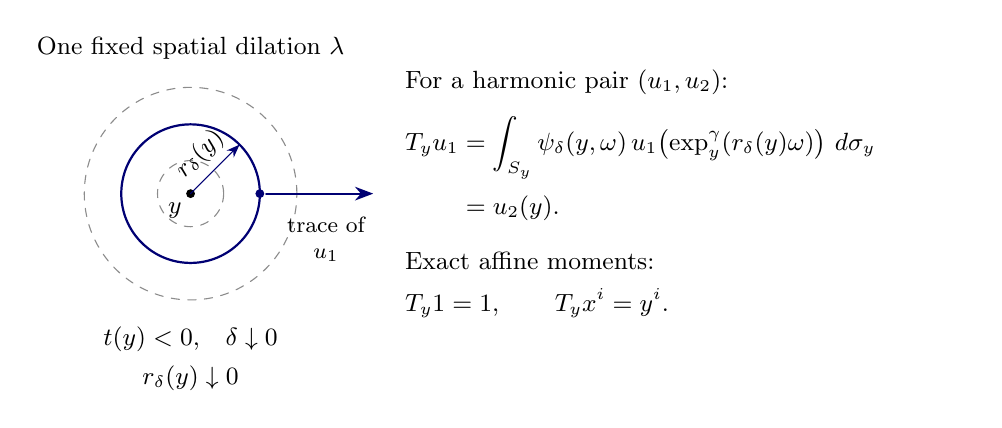
\begin{tikzpicture}[x=1cm,y=1cm,font=\small,>=Stealth,
  line cap=round,line join=round]
  \colorlet{sphereink}{blue!45!black}
  \node at (1.70,2.40) {One fixed spatial dilation $\lambda$};
  \draw[black!45,dashed] (1.70,0.55) circle (1.35);
  \draw[sphereink,thick] (1.70,0.55) circle (0.88);
  \draw[black!45,dashed] (1.70,0.55) circle (0.42);
  \fill (1.70,0.55) circle (1.6pt);
  \node[anchor=north east,inner sep=3pt] at (1.70,0.55) {$y$};
  \draw[->,sphereink] (1.70,0.55)--(2.3223,1.1723);
  \node[rotate=45,anchor=south,inner sep=3pt] at (2.011,0.861) {$r_\delta(y)$};
  \fill[sphereink] (2.58,0.55) circle (1.6pt);
  \draw[->,sphereink,thick] (2.66,0.55)--(4.02,0.55);
  \node[anchor=north,align=center,font=\footnotesize] at (3.42,0.38)
    {trace of\\$u_1$};
  \node[anchor=north,align=center] at (1.70,-1.02)
    {$t(y)<0$,\quad $\delta\downarrow0$\\[3pt]
     $r_\delta(y)\downarrow0$};
  \node[anchor=west,align=left,text width=7.10cm] at (4.30,0.55) {
    For a harmonic pair $(u_1,u_2)$:\\[7pt]
    $\displaystyle
      T_yu_1=\int_{S_y}\psi_\delta(y,\omega)\,
        u_1\!\left(\exp_y^\gamma(r_\delta(y)\omega)\right)
        \,d\sigma_y$\\[5pt]
    $\displaystyle \hphantom{T_yu_1}{}=u_2(y).$\\[9pt]
    Exact affine moments:\\[4pt]
    $\displaystyle T_y1=1,\qquad T_yx^i=y^i.$
  };
\end{tikzpicture}

\caption{A normal-coordinate section of $\gamma$-geodesic spheres in the
first variable, where $\gamma$ is the conformal reference metric.  The
center $y$ satisfies $t(y)<0$.  The spatial dilation $\lambda$ is fixed
while $\delta$ decreases.  The Green functional transfers paired harmonic
functions and reproduces affine harmonic coordinates exactly.  The
unit-sphere measure $d\sigma_y$ has total mass one; the density
$\psi_\delta$ need not be positive.}
\label{fig:shrinking-functional}
\end{figure}

% Derived from OpenAI, September 24, 2026, Apache-2.0.
% Modified October 12, 2026: explicit inputs, attribution, and full-data conclusion.
\section{An estimate on the shrinking spheres}
\label{sec:angular}

The functional in Proposition~\ref{balls:functional} is defined at every positive
radius.  We now estimate its representing density uniformly as the radius
shrinks.  The equation for this density has second-order angular and base
terms.  Comparing a degree-raising operator with a degree-lowering operator
will control both kinds of derivatives; a second comparison will retain the
principal terms caused by the changing metric.

\subsection{The equation for the density}

We use the reference metric $\gamma$, the normalized second principal
matrix $Q$, and $h=Q-\gamma^{-1}$ from
\eqref{balls:normalization}.  In this section the subscript $\delta$ on the positive
radius $r$ is suppressed.  Put
\[
 f=\log r,\qquad \beta=|df|_\gamma.
\]
The required profile bounds are
\begin{equation}\label{angular:profile-bounds}
 \beta\ge\beta_0,\qquad
 \operatorname{Hess}_\gamma f\le-c_0\beta\gamma,
 \qquad |\nabla^j f|\le C_j\beta^j\quad(1\le j\le8),
\end{equation}
where $c_0>0$ and $C_j$ are fixed.  Lemma~\ref{balls:profiles} provides
these bounds with $\beta_0$ arbitrarily large by choosing $p$
sufficiently large.  All background metric bounds
below are on a fixed relatively compact coordinate region; their constants
are uniform in the spatial dilation.

Let $S_\gamma Y$ be the bundle of $\gamma$-unit tangent spheres over the
base region $Y$.  Each sphere has probability measure $d\sigma_y$.
Horizontal differentiation $\nabla$ uses parallel transport for $\gamma$,
including the covariant tensor indices of an operator or section.  This
connection preserves the sphere measure.  Unless otherwise specified, all
norms and full adjoints use $dV_\gamma(y)\,d\sigma_y(\omega)$.

On each tangent unit ball, extend a sphere function harmonically for the
Euclidean metric $\gamma(y)$.  Denote the boundary radial derivative of
this extension by $B$, and its ambient derivatives in an orthonormal frame
by $A_i$.  Thus $B=k$ on the space $\mathcal H_k$ of spherical harmonics
of degree $k$, and $A_i:\mathcal H_k\to\mathcal H_{k-1}$.  The star in
$A_i^*$ denotes the sphere adjoint.  These operators are parallel, with
the indicated tensor indices, and
\begin{equation}\label{angular:elementary-identities}
 [B,A_i^*]=A_i^*,\qquad \sum_i A_i^*A_i^*=0.
\end{equation}
Indeed differentiation lowers homogeneous degree by one, and the second
identity is the adjoint of the vanishing Laplacian of a harmonic extension.
For $s\in\mathbb R$, use the fiber Sobolev norm
\[
 \|v(y,\cdot)\|_s=\|(1+B)^s v(y,\cdot)\|_{L^2(S_y)}.
\]
Lemma~\ref{prelim:spectral-map} gives the angular pseudodifferential
mapping and form bounds in this norm, including the half orders used
below. Tensor-valued versions use the sum over an orthonormal frame.

We write $\Psi^m$ for the classical pseudodifferential operators of order
$m$ on the sphere.  For a positive function $a(y)$, the notation
$a\Psi^m$ means that, after division by $a$, the finitely many symbol and
operator seminorms used below are bounded.  A statement with $j$ base
derivatives permits the indicated additional factor $\beta^j$.

\begin{lemma}[Moving trace operators]\label{angular:trace}
Suppose that the normal balls and the functional $T_y$ of
Proposition~\ref{balls:functional} are defined, and that
\begin{equation}\label{angular:smallness}
 \sum_{|\alpha|\le8}|\partial_y^\alpha h|\le\eps r,
 \qquad r\beta^2\le\eps.
\end{equation}
If $u$ is first-metric harmonic near one such ball, set
\[
 U(y,\omega)=u\bigl(\exp_y^\gamma(r(y)\omega)\bigr).
\]
There are sphere operators $\mathcal C_i$ such that
$\nabla_iU=\mathcal C_iU$.  Their sphere adjoints satisfy
\begin{equation}\label{angular:C-expansion}
 \mathcal C_i^*=r^{-1}A_i^*+f_iB+E_i+F_i,
 \qquad E_i\in r\Psi^1,\quad F_i\in\Psi^0,
 \qquad f_i=\nabla_i f.
\end{equation}
The normalized remainders $r^{-1}E_i$ and $F_i$ have uniform symbol
bounds after up to six base derivatives, with the allowance $C_j\beta^j$.

Write the normalized second equation, in the reference connection, as
$Q^{ij}\nabla_i\nabla_j+b_2^i\nabla_i$.  Its drift $b_2$ is uniformly
controlled.  If $\psi(y,\omega)$ represents $T_y$ against $d\sigma_y$,
then
\begin{equation}\label{angular:P-equation}
 P\psi=0,\qquad
 P=r\left[Q^{ij}(\nabla_i+\mathcal C_i^*)
                    (\nabla_j+\mathcal C_j^*)
             +b_2^i(\nabla_i+\mathcal C_i^*)\right].
\end{equation}
The products in this formula are covariant products.  In particular,
$Q$ is not differentiated by taking a base adjoint.
\end{lemma}

\begin{proof}
Normalize the principal part of the first equation to $\gamma^{-1}$ and
pull it back by $z\mapsto\exp_y^\gamma(rz)$ to the unit ball.  After
multiplication by $r^2$, its principal coefficients are
$\delta^{ij}+O(r^2)$ and its first-order coefficients are $O(r)$.
The resulting smooth family remains uniformly elliptic and has an
invertible Dirichlet problem, including at $r=0$.  Its radial derivative
operator therefore has the expansion
\begin{equation}\label{angular:radial-expansion}
 B+r B_1(y)+r^2 B_2(y,r),\qquad
 B_1\in\Psi^0,\quad B_2\in\Psi^1.
\end{equation}
Here is the parameter justification.  The classical boundary-symbol
construction is described in
\citep[Theorem~1.1(i) and Proposition~3.1]{JoshiLionheart2005};
we keep the center and radius dependence explicitly.
In boundary coordinates the decaying
normal root of the principal symbol constructs the Dirichlet parametrix.
Successive lower-order transport equations construct its symbols smoothly
in $(y,r)$.  The first normal derivative trace is an operator of order one,
whose principal symbol depends only on the principal coefficients and the
differentiating vector.  Those coefficients have zero first $r$-derivative
at $r=0$, so that derivative of the trace operator has order zero.  Taylor's
formula in this symbol class gives \eqref{angular:radial-expansion} to
smoothing error.  The true solution differs from the parametrix by the
Dirichlet inverse of a smooth error; differentiated Dirichlet estimates
control this remainder in every fixed seminorm.  More explicitly, on a
compact center set the rescaled Dirichlet operator is smoothly
invertible between each fixed pair of Sobolev spaces, uniformly for
$0\le r\le r_0$.  Differentiating that inverse controls every fixed
number of parameter derivatives of the smoothing correction; increasing
the Sobolev orders controls its smooth kernel seminorms.  Thus the
Taylor expansion holds in the complete classical symbol topology,
including the smoothing remainder, and not merely in one Sobolev
operator norm.  This proves the stated expansion and its parameter bounds.

Differentiate the exponential map in its center, transporting $\omega$
parallel to the center velocity.  The Jacobi field has initial derivative
zero.  After inverting the differential in the $z$ variable, the velocity
acting on the unit-ball solution is
\[
 r^{-1}\bigl(e_i+O(r^2)\bigr)+f_i\omega.
\]
The coefficient error is smooth in $(y,r,\omega)$.  Tangential derivatives
act directly on the boundary value; the radial derivative is
\eqref{angular:radial-expansion}.  At $r=0$ the first term is $r^{-1}A_i$.
The order-one errors are $O(r)$, and the order-zero errors are bounded:
in particular $r f_i B_1$ is bounded because $r\beta\le\eps/\beta$.
Taking sphere adjoints gives \eqref{angular:C-expansion}.  Differentiating
the radius costs at most one factor $\beta$ per derivative, by
\eqref{angular:profile-bounds}; the asserted parameter estimates follow.

For fixed $u$, differentiate
$T_yu=\langle\psi(y,\cdot),U(y,\cdot)\rangle_{S_y}$.
Metric compatibility and $\nabla_iU=\mathcal C_iU$ put the differentiated
operator on $\psi$ as $\nabla_i+\mathcal C_i^*$.
The local second-metric harmonicity in
Proposition~\ref{balls:functional} proves that
\eqref{angular:P-equation} pairs to zero with the trace of every
function harmonic near the fixed closed ball.  No global extension
or source-family approximation is used in this step.
At a fixed sphere these traces are dense among
smooth boundary data: solve the smooth Dirichlet problem on slightly
enlarged balls, using boundary values transported from the limiting sphere,
and use smooth dependence of the solution on the radius.  Thus the paired
equation is the stated equation for $\psi$.
\end{proof}

\subsection{The model operator and its principal perturbations}

We separate a degree-raising model operator from the remaining
principal and lower-order terms of the moving trace equation.  We continue under the hypotheses of
Lemma~\ref{angular:trace}, including \eqref{angular:smallness}.

Define
\begin{equation}\label{angular:T-definition}
 D_i^+=\nabla_i+f_iB,\qquad D_i^-=-\nabla_i+f_iB,
 \qquad
 T=\sum_i A_i^*D_i^+,\quad T^\flat=\sum_i A_iD_i^-.
\end{equation}
The symbol $T$ here denotes a differential operator on sphere functions;
the transfer functional continues to be denoted $T_y$.
Expand \eqref{angular:P-equation} by
\eqref{angular:C-expansion}.  The identities
\eqref{angular:elementary-identities} give
\[
 D_i^+(r^{-1}A_j^*)=r^{-1}A_j^*D_i^+,
 \qquad \sum_iA_i^*A_i^*=0.
\]
Thus, in ordinary base coordinates and an orthonormal sphere
trivialization,
\begin{equation}\label{angular:P-decomposition}
 P=2T+U+J,
\end{equation}
where $J$ is a uniformly bounded family in $\Psi^1$, with no base
derivatives, and
\begin{equation}\label{angular:U-bounds}
 U=\sum_{|\alpha|\le2}U_\alpha(y)\partial_y^\alpha,
 \qquad U_\alpha\in\eps\beta^{-|\alpha|}
                               \Psi^{2-|\alpha|}.
\end{equation}
Up to five derivatives of these coefficients have the additional
allowance $C_j\beta^j$.  The second-base-derivative term is precisely
\begin{equation}\label{angular:real-principal-part}
 rQ^{ij}\partial_{y_i}\partial_{y_j};
\end{equation}
its coefficients are real scalars independent of the sphere variable.

We detail these bounds.  The pure angular second derivative contracted
with $\gamma^{-1}$ vanishes.  The remaining contraction is
$(h^{ij}/r)A_i^*A_j^*$, and belongs to the zero-base-derivative term of
\eqref{angular:U-bounds}.  The mixed correction is
$2h^{ij}A_i^*D_j^+$ and has the stated small bounds.  The $D^+D^+$ term
has coefficient $r$; its base orders two, one and zero have coefficients
$O(r)$, $O(r\beta)$ and $O(r\beta^2)$, respectively.  The condition
$r\beta^2\le\eps$ gives \eqref{angular:U-bounds} for all three.
Terms containing $E_i$ obey the same bounds.  Terms containing $F_i$
also do so, except for their cross terms with $r^{-1}A_j^*$, which are
bounded angular order-one terms and belong to $J$.  The drift term with
$A_i^*$ belongs to $J$ as well.  Differentiating any of these expressions
gives the stated coefficient bounds by
\eqref{angular:profile-bounds} and \eqref{angular:smallness}.
A horizontal connection written in this trivialization adds a bounded
angular first derivative, which preserves the same estimates.  The bounds
for $J$ use the fixed background and remain uniform as $\beta_0$ is
increased.

The decomposition identifies the model operator $2T$ and the
second-order perturbation $U$.  To carry the model estimate over to $P$
we shall need more than an ordinary first-derivative estimate: the error forms
also contain mixed base and angular derivatives.  For a sphere function
$\varphi$, put
\begin{equation}\label{angular:N-definition}
 \mathcal N(\varphi)^2
 =\int_Y\left(
  \|\nabla\varphi\|_0^2+\beta^2\|\varphi\|_1^2
  +\beta^{-1}\|\nabla\varphi\|_{1/2}^2
  +\beta\|\varphi\|_{3/2}^2\right)dV_\gamma.
\end{equation}

The last two terms of $\mathcal N$ place half an angular derivative
on $\nabla\varphi$ and three halves on $\varphi$.  They will bound the
remaining error forms left by the comparison with $P$.

\subsection{A comparison of raising and lowering operators}

The next estimate supplies these two derivative strengths for the model
operator.  Spherical harmonics are trace-free symmetric tensors, and
the calculation below compares their raising and lowering operators.
Here the negative Hessian of the spatial weight supplies the positive
term that absorbs the bounded curvature.  We give the calculation with
its degree factors.

\begin{lemma}[Weighted raising estimate]\label{angular:raising}
Let $n\ge3$, and suppose \eqref{angular:profile-bounds} holds on a fixed
base region with uniformly bounded reference geometry.  There are
$\beta_0$ and $c>0$, depending only on that geometry and the constants in
\eqref{angular:profile-bounds}, such that every smooth, compactly
base-supported function with zero fiber mean satisfies
\begin{equation}\label{angular:raising-estimate}
 \|T\varphi\|^2-\|T^\flat\varphi\|^2
       \ge c\,\mathcal N(\varphi)^2.
\end{equation}
\end{lemma}

\begin{proof}
Both operators change angular degree by exactly one, so it suffices to
prove the estimate at one input degree $k\ge1$.  Identify that component
with a harmonic homogeneous polynomial $v(z)$ of degree $k$.  Use the
Fischer inner product, in which the monomials $z^\alpha$ are orthogonal
with squared norm $\alpha!$.  Polynomial differentiation $a_i=\partial_{z_i}$
is adjoint to multiplication $M_i=z_i$.  On harmonic polynomials of degree
$k$ the Fischer squared norm is the normalized squared sphere norm
multiplied by
\[
 N_k=n(n+2)\cdots(n+2k-2),\qquad N_0=1.
\]
For completeness, integration against a standard real Gaussian identifies
the Fischer norm on trace-free homogeneous polynomials with their
Gaussian $L^2$ norm;
The Gaussian generating function is $\mathbb E e^{t\cdot X}=e^{|t|^2/2}$.
Its coefficient formula pairs polynomial indices. A pairing within either
trace-free polynomial is zero, so only cross-pairings remain, yielding
$\mathbb E[v(X)\overline{w(X)}]=\sum_\alpha\alpha!v_\alpha\overline{w_\alpha}$.
The radial moment $\mathbb E|X|^{2k}=n(n+2)\cdots(n+2k-2)$
then gives the factor $N_k$.

Set $d=k+n/2-1$ and use $D_i^\pm=\pm\nabla_i+k f_i$ at this fixed degree.
For harmonic polynomials $q_i$ of degree $k$, the Laplacian of
$\sum_iM_iq_i$ is $2\sum_i a_iq_i$.  Since
\[
 \Delta_z(|z|^2s)=4d\,s\qquad(s\in\mathcal H_{k-1}),
\]
its harmonic projection is
$\sum_iM_iq_i-|z|^2\sum_i a_iq_i/(2d)$.  Orthogonality of this projection
and its complement shows that its squared norm is
\[
 \sum_i\|q_i\|^2+\sum_{i,j}(a_jq_i,a_iq_j)
             -d^{-1}\Bigl\|\sum_i a_iq_i\Bigr\|^2.
\]
Changing from Fischer adjoints to sphere adjoints gives
\[
 A_i^*|_{\mathcal H_k}
   =\frac{N_{k+1}}{N_k}\Pi_{k+1}M_i,
\]
where $\Pi_{k+1}$ is harmonic projection in homogeneous degree $k+1$.
Consequently $N_k$ times the left side of
\eqref{angular:raising-estimate} is
\begin{equation}\label{angular:Fock-difference}
 \begin{split}
 (2d+2)\left[\|D^+v\|^2
   +\sum_{i,j}(a_jD_i^+v,a_iD_j^+v)
   -\frac1d\Bigl\|\sum_i a_iD_i^+v\Bigr\|^2\right]
 -2d\Bigl\|\sum_i a_iD_i^-v\Bigr\|^2.
 \end{split}
\end{equation}
All norms in this calculation include integration over the base and use
the polynomial inner product in the fibers.  The factors are
$N_{k+1}/N_k=2d+2$ and $N_k/N_{k-1}=2d$.

Write $C_{ij}=2k(\operatorname{Hess}_\gamma f)_{ij}$ and
\[
 C[av]=\int_Y\sum_{i,j}C_{ij}\langle a_iv,a_jv\rangle\,dV_\gamma.
\]
Covariant integrations by parts give
\begin{align}
 \sum_{i,j}(a_jD_i^+v,a_iD_j^+v)
   &=\Bigl\|\sum_i a_iD_i^-v\Bigr\|^2-C[av]
                                    +O(k^2)\|v\|^2,\label{angular:ibp-one}\\
 \Bigl\|\sum_i a_iD_i^+v\Bigr\|^2
   &\le k\|D^-v\|^2-C[av]+O(k^2)\|v\|^2,\label{angular:ibp-two}\\
 \|D^-v\|^2
   &=\|D^+v\|^2+\int_Y\tr C\,|v|^2\,dV_\gamma.
                                                    \label{angular:ibp-three}
\end{align}
Here and below a form denoted $O(k^2)\|v\|^2$ has absolute value at most
a fixed constant times that quantity.  To verify the first two formulas,
move a $D_j^+$ across the pairing and commute
$D_j^-D_i^+$ to $D_i^+D_j^--C_{ij}$.  The reordered term in
\eqref{angular:ibp-two} is at most $k\|D^-v\|^2$, because
$\sum_i|a_iw|^2=k|w|^2$ for $w\in\mathcal H_k$.
The extra commutator is curvature: it acts as a sum of rotations of norm
$O(k)$ at degree $k$, and the two contractions supply one more factor $k$.
This proves the claimed error bounds.  Expanding the two squares proves
\eqref{angular:ibp-three}.  For complex functions all the displayed forms
are understood through their real parts.

Substituting \eqref{angular:ibp-one} into
\eqref{angular:Fock-difference} rewrites that expression as
\begin{equation}\label{angular:after-first-ibp}
 \begin{split}
 &(2+2/d)\left[d\|D^+v\|^2
       -\Bigl\|\sum_i a_iD_i^+v\Bigr\|^2-dC[av]\right]\\
 &\qquad+2\Bigl\|\sum_i a_iD_i^-v\Bigr\|^2
                      +O(k^3)\|v\|^2.
 \end{split}
\end{equation}
We must control the remaining negative divergence square while retaining
both an ordinary derivative estimate and an additional half-order
angular derivative estimate.  The latter requires a coefficient of
size $k/\beta$ in front of $|D^+v|^2$, including when $k$ is much larger
than $\beta$.  Choose a small constant $\vartheta>0$.
On the fraction $1-\vartheta$ of its negative divergence square use
\eqref{angular:ibp-two}--\eqref{angular:ibp-three}.  On the remaining
fraction use the pointwise convex combination
\begin{equation}\label{angular:convex-bound}
 \begin{split}
 \Bigl|\sum_i a_iD_i^+v\Bigr|^2
 &\le(1-\zeta)(k+n-1)|D^+v|^2\\
 &\quad+\zeta\left(2\Bigl|\sum_i a_iD_i^-v\Bigr|^2
                         +8k^3\beta^2|v|^2\right),
 \qquad \zeta=c_1/\beta.
 \end{split}
\end{equation}
The fraction $1-\vartheta$ in the integrated estimates is constant;
the $y$-dependent $\zeta$ is used only in this pointwise inequality.
The first bound follows from the adjoint multiplication operators, since
the contraction $(q_i)\mapsto\sum_i a_iq_i$ has squared norm at most
$k+n-1$ on polynomials of degree $k$.  The second follows from
$D_i^++D_i^-=2k f_i$ and
$|\sum_i f_i a_i v|^2\le k\beta^2|v|^2$.

Combining these bounds in \eqref{angular:after-first-ibp}, the coefficient
retained for $|D^+v|^2$ is
\begin{equation}\label{angular:positive-degree-factor}
 (2+2/d)\bigl[d-k-\vartheta(n-1)
                         +\vartheta\zeta(k+n-1)\bigr].
\end{equation}
Since $d-k=(n-2)/2$, a sufficiently small fixed $\vartheta$ makes this
at least a fixed positive constant plus a positive multiple of
$c_1k/\beta$.  The coefficient of
$|\sum_i a_iD_i^-v|^2$ is nonnegative when $\beta_0$ is sufficiently
large.  The Hessian contribution is exactly
\begin{equation}\label{angular:hessian-contribution}
 -(2+2/d)\left[(d-1+\vartheta)C[av]
       +(1-\vartheta)k\int_Y\tr C\,|v|^2\,dV_\gamma\right].
\end{equation}
For $k\ge1$ and $n\ge3$, both coefficients inside this expression are
positive.  The Hessian hypothesis bounds it below by
$c k^3\int\beta|v|^2$.  This absorbs the curvature error $O(k^3)\|v\|^2$
by increasing $\beta_0$, and absorbs the last term of
\eqref{angular:convex-bound} by choosing $c_1$ sufficiently small.
We have therefore retained positive multiples of
\[
 \|D^+v\|^2,\qquad
 \int_Y\frac{k}{\beta}|D^+v|^2\,dV_\gamma,
 \qquad k^3\int_Y\beta|v|^2\,dV_\gamma.
\]
The first controls both $\|\nabla v\|^2$ and
$k^2\int\beta^2|v|^2$, since its cross term is
$-k\int\Delta_\gamma f\,|v|^2\ge0$.  For the weighted derivative use the
pointwise inequality
\[
 \frac{k}{\beta}|\nabla v|^2
 \le2\frac{k}{\beta}|D^+v|^2+2k^3\beta|v|^2.
\]
No differentiation of $\beta^{-1}$ is required.  Dividing by $N_k$, and
then summing the orthogonal degree components, proves
\eqref{angular:raising-estimate}; the weights $(1+k)^s$ are comparable
to $k^s$ because the zero degree is excluded.
\end{proof}

\subsection{Keeping the principal perturbations}

The raising estimate controls the model operator.  The actual equation
\eqref{angular:P-equation} also contains second base derivatives and a
small second-order angular perturbation.  We retain these terms in a
comparison of squared norms.

\begin{proposition}[Coercivity for the moving trace equation]
\label{angular:coercivity}
Fix a base region with bounded reference geometry and the constants in
\eqref{angular:profile-bounds}.  Suppose $P$ is the operator
\eqref{angular:P-equation}, with the trace operators of
Lemma~\ref{angular:trace}.  There exist $\beta_0$ sufficiently large,
$\eps_0>0$ and $C<\infty$, depending only on these fixed bounds, such that
\eqref{angular:smallness} with $\eps\le\eps_0$ implies
\begin{equation}\label{angular:coercive-estimate}
 \mathcal N(\varphi)\le C\|P\varphi\|
\end{equation}
for every smooth, compactly base-supported function $\varphi$ with
zero mean on each sphere.  These constants are independent of the
shrinking parameter.  Only the eight indicated derivatives of the small
tensor $h$ are required.
\end{proposition}

\begin{proof}
Let a dagger denote the full adjoint for $dV_\gamma d\sigma$.
Covariant integration and the degree shift give
\begin{equation}\label{angular:Z-definition}
 Z:=T^\flat-T^\dagger=\sum_i f_iA_i.
\end{equation}
A direct expansion yields
\begin{equation}\label{angular:norm-comparison}
 \begin{split}
 &\|(2T+U)\varphi\|^2-
                \|(2T^\flat+U^\dagger)\varphi\|^2\\
 &\qquad=4\bigl(\|T\varphi\|^2-\|T^\flat\varphi\|^2\bigr)
                       +\langle\mathcal E\varphi,\varphi\rangle,
 \end{split}
\end{equation}
where
\begin{equation}\label{angular:error-operator}
 \mathcal E=2[T^\dagger,U]+2[U^\dagger,T]+[U^\dagger,U]
                       -2\bigl(UZ+(UZ)^\dagger\bigr).
\end{equation}
We will prove
\begin{equation}\label{angular:error-form-bound}
 |\langle\mathcal E\varphi,\varphi\rangle|
                         \le C\eps\mathcal N(\varphi)^2.
\end{equation}

Here are the complete order and weight counts needed for this claim.
An operator has count $(m,s)$ if its coefficient at $\partial_y^\alpha$
is angular order $m-|\alpha|$, of size $O(\beta^{s-|\alpha|})$,
with the derivative allowances already specified.
Adjoints preserve the count, and products add the counts.  When a base
derivative hits a coefficient it consumes one differential order and
adds a factor $\beta$, so it preserves the weight index.  A commutator
of scalar angular operators loses one angular order: the products of
their principal symbols cancel.  Hence a scalar commutator loses one in
total order while preserving the sum of the weight indices.
The counts of $T,T^\dagger,U,Z$ are, respectively,
\[
 (2,1),\quad(2,1),\quad(2,0),\quad(1,1),
\]
and every occurrence of $U$ carries the factor $\eps$.  Thus
\eqref{angular:error-operator} has count at most $(3,1)$ and a factor
$O(\eps)$; the quadratic $U$ term is smaller.

There is a further cancellation that the total count alone does not
express: no third base derivative survives.  To check it explicitly,
use an orthonormal sphere trivialization and write the base measure as
$\mu(y)\,dy$.  The sphere probability measure is then fixed.  Write
\[
 U=a^{ij}\partial_i\partial_j+\mathcal B^i\partial_i+\mathcal C,
 \qquad a^{ij}=rQ^{ij}=a^{ji}\in\mathbb R.
\]
The coefficients $\mathcal B^i$ and $\mathcal C$ are angular
operators.  Replacing a horizontal derivative by a coordinate derivative
plus its angular connection term changes only base orders at most one,
so these are all the second-base coefficients.  If a star denotes the
sphere adjoint, direct integration by parts gives
\begin{align*}
 U^\dagger-U
 ={}&\left(2\mu^{-1}\partial_j(\mu a^{ij})
                -\mathcal B^i-(\mathcal B^i)^*\right)\partial_i\\
 &+\mu^{-1}\partial_i\partial_j(\mu a^{ij})
       -\mu^{-1}\partial_i\bigl(\mu(\mathcal B^i)^*\bigr)
       +\mathcal C^*-\mathcal C.
\end{align*}
In particular it has base order at most one.
In $[T^\dagger,U]$ and
its partner, the possible third-base-derivative coefficient is a commutator of an angular coefficient
with $rQ^{ij}$, which is zero by
\eqref{angular:real-principal-part}.  For $[U^\dagger,U]$, first write
it as $[U^\dagger-U,U]$.  The operator $U^\dagger-U$ has no second base
derivative, since the coefficient in
\eqref{angular:real-principal-part} is real.  Taking adjoints against
the smooth base density only produces lower base orders.  Its remaining
possible third-base-derivative coefficients commute for the same reason.
Finally, $UZ$ already has at most two base derivatives.
It follows that $\mathcal E$ is a sum of terms of precisely the following
three permitted types:
\begin{equation}\label{angular:error-types}
 \eps\beta^{-1}\Psi^1\partial_y^2,
 \qquad \eps\Psi^2\partial_y,
 \qquad \eps\beta\Psi^3.
\end{equation}
This argument also covers lower orders, since $\beta\ge1$.

For the first type in \eqref{angular:error-types}, integrate once in the
base.  The principal form is bounded by
$C\eps\int\beta^{-1}\|\partial_y\varphi\|_{1/2}^2$.
A derivative of its coefficient costs one factor $\beta$ and leaves an
$\eps\Psi^1\partial_y$ term.  This includes differentiation of the
weight itself: $|d\beta|\le C\beta^2$ implies
$|d(\beta^{-1})|\le C$.  The second type has the form bound
\[
 C\eps\int_Y
     \|\partial_y\varphi\|_{1/2}\|\varphi\|_{3/2}\,dV_\gamma
 \le C\eps\int_Y\left(
     \beta^{-1}\|\partial_y\varphi\|_{1/2}^2
                 +\beta\|\varphi\|_{3/2}^2\right)dV_\gamma.
\]
The third type is bounded by
$C\eps\int\beta\|\varphi\|_{3/2}^2$.
The lower-order term from differentiating a coefficient satisfies the
same bound.  Replacing coordinate derivatives by horizontal derivatives
adds a bounded angular first derivative, again controlled by these norms.
A fixed finite partition of the base region has the same harmless
lower-order errors.  This proves \eqref{angular:error-form-bound}.

The constants in the preceding estimates are uniform for all
$\beta\ge\beta_0$ once a fixed lower threshold is met.  Choose
$\eps_0$ small relative to the constant in
Lemma~\ref{angular:raising}.  Dropping the nonnegative second squared
norm in \eqref{angular:norm-comparison} gives
$\mathcal N(\varphi)\le C\|(2T+U)\varphi\|$.
Finally,
\[
 \|J\varphi\|\le C\|\varphi\|_{L^2(Y;H^1(S_y))}
                         \le C\beta_0^{-1}\mathcal N(\varphi),
\]
so a sufficiently large $\beta_0$ absorbs $J$ and proves
\eqref{angular:coercive-estimate}.

All these operations use angular symbol estimates pointwise in the base,
and ordinary base differential operators of degree at most two.  Formal
adjoints, the commutator expansion and the one integration by parts use
at most the five base coefficient derivatives specified in
\eqref{angular:U-bounds}.  Construction of these coefficients differentiates
the moving trace operators once and the second metric to only finitely
many orders below eight.  Higher angular symbol seminorms depend on the
fixed smooth first-metric family; differentiating in the angular variable
does not differentiate the center-dependent tensor $h$.  Thus the eight
smallness derivatives in \eqref{angular:smallness} suffice in every fixed
dimension.  No smallness assumption on all derivatives of $h$ is used.
\end{proof}

\subsection{The constant mode and the uniform density bound}

We now apply the coercive estimate to the transfer density constructed in
Section~\ref{sec:balls}, restoring the notation $r=r_\delta$.
Its normalization is $\int_{S_y}\psi\,d\sigma_y=1$, so
$\chi(\psi-1)$ has zero fiber mean for the fixed cutoff
\eqref{balls:cutoff-region}.  This is the mean-zero condition required
by Proposition~\ref{angular:coercivity}.

The decomposition \eqref{angular:P-decomposition} gives a uniform
bound for $P1$: its raising part annihilates $1$, only $U$'s bounded
zero-base-derivative coefficient acts on $1$, and $J$ is uniformly
bounded in $\Psi^1$.  There is no factor growing with $\beta$ in this
assertion.

For any fixed smooth base cutoff, the same decomposition gives
\begin{equation}\label{angular:cutoff-bound}
 \|[P,\chi]w\|
 \le C_\chi\left(
  \|w\|_{L^2(\supp d\chi;H^1(S_y))}
    +\|r\nabla w\|_{L^2(\supp d\chi\times S_y)}\right),
\end{equation}
where the support can be replaced by a fixed small neighborhood of the
supports of all derivatives of $\chi$.
Indeed $[2T,\chi]=2\sum_iA_i^*(\nabla_i\chi)$, the second base derivative
of $U$ contributes $2rQ^{ij}(\partial_i\chi)\partial_j$ and a bounded
zeroth-base-derivative term, and its first base derivative contributes a
bounded angular order-one term.  The operator $J$ commutes with $\chi$.

\begin{lemma}[Uniform transfer density]\label{local:density}
Fix the structural parameters so that Propositions
\ref{balls:continuation} and \ref{angular:coercivity} apply.  There is
a constant $C$ independent of $\delta$ and of sufficiently small
spatial dilations $\lambda$ such that
\begin{equation}\label{local:density-bound}
 \|\chi\psi\|_{L^2(S_\gamma Y)}\leq C
\end{equation}
whenever the coefficient condition
\eqref{balls:bootstrap-condition} holds.
\end{lemma}

\begin{proof}
Set $\varphi=\chi(\psi-1)$, which is compactly supported in the base
and has zero fiber mean.  For the actual moving-sphere operator $P$,
Equation~\eqref{angular:P-equation} gives
\begin{equation}\label{local:density-equation}
 P\varphi=P\bigl(\chi(\psi-1)\bigr)
       =-\chi P1+[P,\chi](\psi-1).
\end{equation}
The cutoff estimate \eqref{angular:cutoff-bound} involves only angular
derivatives through order one and $r\nabla\psi$ on the supports of
derivatives of $\chi$.  Proposition~\ref{balls:functional} bounds
these there uniformly: on the lower region the density is that of
ordinary evaluation, and on the other region the radii stay at a fixed
positive separation.  Together with the bound for $P1$, this gives a
uniformly bounded $L^2$ norm for the right side of
\eqref{local:density-equation}.
Proposition~\ref{angular:coercivity} bounds $\varphi$; adding the fixed
function $\chi$ proves \eqref{local:density-bound}.
\end{proof}

The uniform bound now applies to the density representing the actual
Green functional at every radius allowed by
\eqref{balls:bootstrap-condition}.  Exact affine moments will turn it
into a two-power bound for the paired harmonic differences.

% Derived from OpenAI, September 24, 2026, Apache-2.0.
% Modified October 12, 2026: explicit inputs, attribution, and full-data conclusion.
\section{From harmonic differences to local metric extension}\label{sec:bootstrap}

Lemma~\ref{local:density} bounds the transfer density uniformly on the
shrinking spheres.  Exact reproduction of affine functions now turns that
bound into a two-power estimate for the difference of paired harmonic
functions.  The harmonic Hessians convert derivatives of these differences
into metric derivatives.  Finite-order interpolation will then improve
the temporary metric bound and allow the radii to shrink with the spatial
dilation held fixed.

\subsection{From the functional to harmonic jets}

Return to the finite harmonic family in Theorem~\ref{local:extension}.
Its values and first derivatives at $0$ agree between the two metrics,
because the functions agree on the one-sided open set and are smooth.
After dilation define
\begin{equation}\label{local:renormalized-pairs}
 v_{j,\lambda}^a(y)=\lambda^{-2}
 \bigl(u_j^a(\lambda y)-u_1^a(0)
                     -\lambda\,du_1^a(0)\cdot y\bigr).
\end{equation}
The subtracted functions are harmonic because the coordinates are
harmonic.  These new pairs still agree on the known side and are
transferred by $T_y$.  For each fixed integer $m$ they have uniform
$C^m$ bounds on every required fixed bounded coordinate neighborhood.
For derivative orders $j\geq2$, this follows from the factor
$\lambda^{j-2}$; orders zero and one follow from the second-order
Taylor remainder.  Moreover,
\[
 \partial^2v_{1,\lambda}^a(y)\longrightarrow\partial^2u_1^a(0)
\]
smoothly on fixed sets.  Thus the Hessian spanning condition has a
uniform rank bound after sufficiently small dilation.  Write
$V^a=v_{2,\lambda}^a-v_{1,\lambda}^a$.

\begin{lemma}[Two-power moment bound]\label{local:moment}
Under the coefficient condition \eqref{balls:bootstrap-condition},
the paired differences satisfy
\begin{equation}\label{local:moment-bound}
 \left\|\frac{\chi V^a}{r_\delta^2}\right\|_{L^2(Y)}\leq C
\end{equation}
with a constant independent of $\delta$ and sufficiently small
$\lambda$.
\end{lemma}

\begin{proof}
Fix a center $y$ and subtract from $v_{1,\lambda}^a$ its affine
coordinate Taylor polynomial at $y$.  Exact constant and coordinate
reproduction in \eqref{balls:reproduction} cancels this polynomial in
$T_yv_{1,\lambda}^a-v_{1,\lambda}^a(y)=V^a(y)$.  The remainder on
$\partial B_\gamma(y,r)$ is bounded by $Cr^2$, since coordinate
distance and $\gamma$-distance are uniformly comparable and the
functions have uniform second derivatives.  Hence
\[
 |V^a(y)|\leq C r_\delta(y)^2
                         \|\psi(y,\cdot)\|_{L^2(S_y)}.
\]
Lemma~\ref{local:density} proves \eqref{local:moment-bound}.  The
coordinate volume measure and $dV_\gamma$ are uniformly comparable.
No derivative in $y$ of the continued density is used here.
\end{proof}

We next express metric derivatives in terms of derivatives of the paired
differences.  Recovery of the conformal metric
class from the hyperplane of harmonic Hessians is also used in
\citep[Proposition~4.1 and Remark~4.2]{LLS20}.
All Hessians in this step are
ordinary coordinate Hessians, not covariant Hessians.  Because the
coordinates are harmonic, the equations for $v_{j,\lambda}^a$ have
no first-order term in these coordinates:
\[
 (g_{k,\lambda}^{-1})^{ij}\partial_{ij}v_{k,\lambda}^a=0
 \qquad(k=1,2).
\]
Multiplication by the scalar factors in
\eqref{balls:normalization} therefore gives
\begin{equation}\label{local:metric-system}
 h^{ij}\partial_{ij}v_{1,\lambda}^a
       =-Q^{ij}\partial_{ij}V^a,
 \qquad \operatorname{tr}(\gamma h)=0.
\end{equation}

Harmonicity puts each $\partial^2v_{1,\lambda}^a(y)$ in the hyperplane
annihilated by $\gamma^{-1}(y)$.  The uniform rank bound established
above shows that these matrices span this hyperplane for small $\lambda$.  The extra equation
$\operatorname{tr}(\gamma h)=0$ completes an injective system on
symmetric contravariant matrices: an element annihilating all those
Hessians is a multiple of $\gamma^{-1}$, and its $\gamma$-trace is
$n$ times that multiple.  The associated finite matrix has a smooth
left inverse with uniform derivatives on $Y$.  For example, in fixed
coordinate bases use $(A^*A)^{-1}A^*$, where $A$ is this injective
matrix.  Its smallest singular value stays bounded below by the
spanning condition and smooth convergence under dilation.
Differentiating \eqref{local:metric-system} at most eight times gives
\begin{equation}\label{local:metric-jet-bound}
 H_8(y)\leq C\sum_a\sum_{|\alpha|\leq10}
                              |\partial^\alpha V^a(y)|.
\end{equation}
The derivatives of $Q$, $\gamma$, and of the finite harmonic family
are uniformly bounded.  In particular, this inversion introduces no
factor involving $r_\delta^{-1}$.

The metric estimate requires derivatives of the paired differences
through order ten, whereas Lemma~\ref{local:moment} controls only their
weighted $L^2$ norm.  The following finite-order interpolation estimate
bridges these two statements using the already fixed smooth bounds.

\begin{lemma}[Finite-order interpolation]\label{local:interpolation}
Let $V$ be smooth on a neighborhood of $\overline{B(y,s)}\subset
\mathbb R^n$, with $0<s\leq1$ and $\|V\|_{C^m}\leq A_m$ there.
For every multi-index $\alpha$ of length $j<m$,
\begin{equation}\label{local:interpolation-estimate}
 |\partial^\alpha V(y)|\leq C_{m,n}
 \bigl(s^{-j-n/2}\|V\|_{L^2(B(y,s))}
                          +A_m s^{m-j}\bigr).
\end{equation}
\end{lemma}

\begin{proof}
Expand $V(y+sz)$ at $z=0$ through degree $m-1$ on the unit ball.
The remainder has absolute value at most $C_{m,n}A_m s^m$.
The $L^2$ norm of the Taylor polynomial is therefore at most
$s^{-n/2}\|V\|_{L^2(B(y,s))}+C_{m,n}A_m s^m$.
On the finite-dimensional space of polynomials of degree at most
$m-1$, every coefficient is bounded by a constant times the $L^2$
norm on the unit ball.  Its $z^\alpha$ coefficient is
$s^j\partial^\alpha V(y)/\alpha!$, giving the claim.
\end{proof}

\subsection{A strict improvement of the metric bound}

Set
\begin{equation}\label{local:exponents}
 D=10+n/2,\qquad \eta=\frac1{2D},\qquad
 p>2D,\qquad m\geq\lceil10+3D\rceil.
\end{equation}
We also take the integer $p$ large enough for
Proposition~\ref{angular:coercivity}.  Thus $\eta>1/p$, and $m$ is
one fixed finite smoothness order.  The constants may depend on these
choices, which precede the final spatial dilation and all shrinkage.

\begin{lemma}[Superlinear improvement]\label{local:improvement}
After the choices in \eqref{local:exponents}, there are $C>0$ and
$\rho_0>0$, independent of $\delta$ and sufficiently small $\lambda$,
such that the coefficient condition
\eqref{balls:bootstrap-condition} implies
\begin{equation}\label{local:superlinear}
 H_8(y)\leq C r_\delta(y)^{3/2}
 \quad\text{for }y\in K\text{ with }r_\delta(y)<\rho_0.
\end{equation}
\end{lemma}

\begin{proof}
Put $r=r_\delta(y)$ and $s=r^\eta$.  By
Lemma~\ref{balls:profiles}, $r_\delta^{1/p}$ has a fixed Lipschitz
constant.  Since
\[
 \frac{s}{r^{1/p}}=r^{\eta-1/p}\longrightarrow0,
\]
a sufficiently small threshold $\rho_0$ ensures
\[
 \tfrac12 r^{1/p}\leq r_\delta(z)^{1/p}
                         \leq\tfrac32 r^{1/p}
             \quad(z\in B(y,s)).
\]
The same fixed threshold ensures that this ball lies where $\chi=1$,
because $K$ has a fixed buffer inside that set.  The upper comparison
and Lemma~\ref{local:moment} imply
\[
 \|V^a\|_{L^2(B(y,s))}\leq C r^2.
\]
Apply Lemma~\ref{local:interpolation} and the fixed uniform $C^m$
bounds of the renormalized functions.  For $j\leq10$ it gives
\[
 |\partial^\alpha V^a(y)|
   \leq C_m\bigl(r^{2-\eta(j+n/2)}+r^{\eta(m-j)}\bigr)
   \leq C_m r^{3/2}.
\]
Both exponents are at least $3/2$ by \eqref{local:exponents}.
Equation~\eqref{local:metric-jet-bound} completes the proof.
\end{proof}

The gain in \eqref{local:superlinear} is stronger than the temporary
bound $H_8\leq\varepsilon r_\delta$.  Its usefulness is that a single
choice of the spatial dilation makes the improvement strict at every
radius, including those above the small threshold.

\subsection{Local extension of the isometry}

\begin{proof}[Proof of Theorem~\ref{local:extension}]
Make the linear normalization and spatial dilation of
Section~\ref{sec:balls}.  All harmonic functions and their finite
spanning family are chosen before the dilation.  We now specify the
remaining choices and hold each one fixed before making the next.

First choose the fixed conformal geometry, cylinder, depth function,
and cutoff, keeping uniform background smooth bounds for
$0<\lambda\leq\lambda_0$.  Choose $p,\eta,m$ as in
\eqref{local:exponents}, with $p$ large enough for the geometric and
angular estimates.  Choose $\varepsilon$ for those estimates and then
$R_*$ so that the balls lie in normal neighborhoods and
$r_\delta\beta_\delta^2\leq\varepsilon$ for every $\delta$.
These choices fix every separation range needed to start the
continuation and to bound the cutoff terms.  Restrict $\lambda_0$
further so that Proposition~\ref{cross:initial} applies to these fixed
ranges, with bounds uniform for $0<\lambda\leq\lambda_0$.

The constants $C,\rho_0$ of Lemma~\ref{local:improvement} are now
fixed.  Choose
\begin{equation}\label{local:rho-choice}
 0<\rho<\rho_0,\qquad C\rho^{1/2}\leq\varepsilon/2.
\end{equation}
At points with $r_\delta<\rho$, that lemma improves the coefficient
bound to $H_8\leq\varepsilon r_\delta/2$ whenever the temporary bound
holds.  At points with $r_\delta\geq\rho$, the same improvement will
hold if
\begin{equation}\label{local:one-dilation}
 \sup_Y H_8\leq\varepsilon\rho/2.
\end{equation}
Since $h\to0$ smoothly under dilation, choose one
$\lambda\leq\lambda_0$ satisfying \eqref{local:one-dilation} and the
additional initial bounds described next.  This $\lambda$ is kept
fixed for the rest of the proof.

There is a uniform reason the coefficient bound holds off $K$ for
every $\delta$.  Outside $K$, either $y_n<-1/2$, where $h=0$ after
the fixed dilation is sufficiently small, or $t>2t_b$, where
\[
 r_\delta\geq R_*(2t_b)^p>0.
\]
Smooth smallness of $h$ therefore gives
$H_8\leq\varepsilon r_\delta/2$ off $K$ for every $\delta$ by
reducing the same dilation once.  At $\delta=1$, the radius has a
positive minimum on all of $Y$, so we can also ensure the initial
coefficient bound there.  These conditions involve only fixed
positive constants, and are compatible with
\eqref{local:one-dilation}.

For this fixed metric pair on the dilated neighborhood, set
\[
 \mathcal A=\{\delta\in(0,1]:
        H_8(y)\leq\varepsilon r_\delta(y)\text{ for every }y\in K\}.
\]
It contains $1$.  At any $\delta\in\mathcal A$, the bound already
established off $K$ gives the full hypothesis
\eqref{balls:bootstrap-condition}.  Proposition~\ref{balls:continuation}
and the uniform density estimate of Lemma~\ref{local:density} then apply.
The moment bound, metric system, and interpolation argument give
Lemma~\ref{local:improvement}.
The small-radius improvement \eqref{local:rho-choice} and the
large-radius bound \eqref{local:one-dilation} give
\[
 H_8\leq\tfrac12\varepsilon r_\delta\quad\text{on }K.
\]
For every fixed positive $\delta$, $r_\delta$ has a positive minimum
on the compact set $K$.  Thus
$\delta\mapsto\max_K(H_8/r_\delta)$ is continuous on $(0,1]$.
The set $\mathcal A$ is relatively closed, and the strict improvement
makes it relatively open.  Connectedness implies
$\mathcal A=(0,1]$.

Finally let $\delta\downarrow0$, with the spatial dilation, harmonic
family, cutoff and all structural parameters fixed.  On the fixed
open neighborhood of $0$ where $t<0$, the radii tend to zero.  Hence
$h=0$ there.  By \eqref{balls:normalization}, $g_{2,\lambda}$ is
conformal to $g_{1,\lambda}$ on that neighborhood.  Write
$g_{2,\lambda}=e^{2\omega}g_{1,\lambda}$.  The conformal change formula
for the Laplace--Beltrami operator is
\[
 \Delta_{e^{2\omega}g}u
  =e^{-2\omega}\bigl(\Delta_g u
                 +(n-2)\langle d\omega,du\rangle_g\bigr).
\]
Apply it to every common harmonic coordinate.  Since their
differentials form a basis and $n-2\ne0$, it forces $d\omega=0$.
Since $g_{1,\lambda}(0)=g_{2,\lambda}(0)=I$, this constant is zero.
This direct conformal calculation also appears in
\citep[Proposition~4.1]{LLS20}.
The metrics therefore agree on a connected neighborhood of $0$;
undoing the dilation proves the theorem.
\end{proof}

For clarity, the two limits in this proof have different roles:
spatial dilation is used once to obtain a fixed small metric
difference, and the subsequent shrinking family improves the bound
for that same difference.  The parameter order is
\begin{equation}\label{local:parameter-order}
 \begin{gathered}
 \text{fixed geometry and harmonic family}
   \;\longrightarrow\;(p,\eta,m)
   \;\longrightarrow\;(\varepsilon,R_*)\\
 \longrightarrow\;\rho\;\longrightarrow\;
 \lambda\text{ fixed}\;\longrightarrow\;\delta\downarrow0.
 \end{gathered}
\end{equation}
All estimates use finitely many derivatives selected before either
limiting step.  Theorem~\ref{local:extension} is the local input that
will prevent a maximal matched region from having an interior
frontier.

% Derived from OpenAI, September 24, 2026, Apache-2.0.
% Modified October 12, 2026: explicit inputs, attribution, and full-data conclusion.
\section{The global isometry and the measured boundary}
\label{global:section}

We now apply Theorem~\ref{local:extension} to the data constructed in
Section~\ref{data:section}. The source evaluations identify which
points should correspond. Their separation makes this correspondence
single-valued, and their behavior at the boundary prevents its escape
from the interior. The local theorem then removes every interior
frontier of the isometric correspondence.
The use of a maximal matching set and limits of source evaluations
follows the source-embedding architecture in
\citep[Section~6.1]{LLS20}; Theorem~\ref{local:extension} supplies the
smooth continuation step needed here.

Retain the extended manifolds $M_j^e$, their common cap $E$, the open
source set $U_0\Subset E$, and the functionals $I_j$ of
Equation~\eqref{data:evaluations}. For this section an \emph{admissible
match} is a smooth local isometry
\[
 \Phi:W\longrightarrow (M_1^e)^\circ,
 \qquad W\subset(M_2^e)^\circ,
\]
where $W$ is connected, open, and contains $E$, such that
\begin{equation}\label{global:matching}
 \Phi|_E=\Id,\qquad I_2(p)=I_1(\Phi(p))\quad(p\in W).
\end{equation}
Thus $\Phi^*g_1=g_2$ on $W$. The identity on $E$ is an admissible
match by Proposition~\ref{data:cap}.

\begin{proposition}[No interior frontier]\label{global:frontier}
There is an isometry
\[
 \Phi:(M_2^e)^\circ\longrightarrow(M_1^e)^\circ
\]
onto the first interior satisfying Equation~\eqref{global:matching}.
\end{proposition}

\begin{proof}
\emph{The maximal match and its Green kernel.}\quad
Two admissible matches agree wherever their domains overlap, since
$I_1$ separates interior points by Lemma~\ref{data:jet-family}.
Their union therefore defines a single smooth local isometry on
the union $W$ of all admissible domains. This union is connected
because every domain contains the connected set $E$. The union
map is injective: equal images give equal $I_2$ evaluations, hence
equal original points. It is itself an admissible match and is
maximal by construction.

We first record the Green equality on this larger region:
\begin{equation}\label{global:green-equality}
 G_2(p,q)=G_1(\Phi(p),\Phi(q)),
             \qquad p,q\in W,\quad p\ne q.
\end{equation}
For fixed $p\in W$, equality of its evaluations and the common
source density give this equality for the other variable in $U_0$,
initially in the distributional sense. Both Green functions are
smooth away from their pole. After pullback by the local isometry,
their difference is harmonic on $W\setminus\{p\}$. This set is
connected, and equality holds on a nonempty open part of it.
Unique continuation proves Equation~\eqref{global:green-equality}.

\emph{A frontier partner and common coordinates.}\quad
Suppose $W$ is not the entire second interior. Connectedness gives
an interior frontier point $p$. If $p_k\in W$ tends to $p$,
compactness of $M_1^e$ gives a subsequential limit $q$ of
$\Phi(p_k)$. For every fixed source $f$, continuity up to the
boundary gives
\[
 I_2(p)(f)=I_1(q)(f).
\]
The point $q$ is interior: all boundary evaluations are zero,
whereas $I_2(p)$ is nonzero. Any two such limits have the same
evaluations and so coincide. It follows that every matched sequence
tending to $p$ has partners tending to this unique $q$.
In particular, nearby matched points have partners in any prescribed
neighborhood of $q$.

Both $p$ and $q$ are outside $\overline{U_0}$. The first statement
holds because $\overline{U_0}\subset E\subset W$. If $q$ belonged
to $\overline{U_0}$, the common-cap identification would give
$I_1(q)=I_2(q)$; separation on the second manifold would force
$p=q\in E$, a contradiction.

Choose sources $f_1,\ldots,f_n$ so that
\[
 y=(u_{f_1}^2,\ldots,u_{f_n}^2)
\]
has independent differentials at $p$, and put
$x=(u_{f_1}^1,\ldots,u_{f_n}^1)$ near $q$.
The second tuple is also a coordinate system. Indeed the isometries
at the points $p_k$ give equality of the gradient Gram matrices
\[
 \bigl(\langle du_{f_a}^2,du_{f_b}^2\rangle_{g_2}(p_k)\bigr)_{a,b}
 =
 \bigl(\langle du_{f_a}^1,du_{f_b}^1\rangle_{g_1}(\Phi(p_k))\bigr)_{a,b}.
\]
The first limit is positive definite, and so is the second.
The coordinate values at $p,q$ coincide. Restricting the charts
gives a common coordinate ball $V$ about this value, with closures
away from $\overline{U_0}$. The preceding convergence observation
ensures that every already matched point sufficiently near $p$
has its partner in the first chart. In these coordinates its
identification is $x=y$.

Let $A\subset V$ be the coordinate image of the already matched
second-side points. It is open and has the center value in its
relative frontier. The two coordinate metrics and every paired
source function agree on $A$. By Lemma~\ref{data:jet-family},
choose finitely many first-side source functions whose ordinary
Hessians span the hyperplane annihilated by $g_1^{-1}$ at the
center. After shrinking $V$, their spanning rank has a positive
lower bound throughout $V$. Their second-side partners are
harmonic there and agree with them on $A$.

\emph{A touching ball removes the frontier.}\quad
We can now find a smooth ball touching the unknown part, without
assuming any regularity of the frontier of $A$. Choose $c\in A$
sufficiently close to the center that
\[
 r=\dist(c,V\setminus A)>0,\qquad
 \overline{B(c,r)}\Subset V.
\]
For example, if the center has distance $R$ from $\partial V$,
take $c$ within $R/3$ of it. Then $r<R/3$, and a minimizing
sequence stays in a compact subset of $V$. Thus the distance is
attained at some
\[
 z_*\in\partial B(c,r)\cap(V\setminus A).
\]
On $B(c,r)$ the metrics, the finite harmonic pairs, and the Green
kernels in both variables agree. Smoothness gives equality of
the metric and harmonic-function jets at $z_*$, and the Hessian spanning
condition holds there by our choice of $V$. All the inputs of
Theorem~\ref{local:extension} are therefore satisfied at $z_*$.
It gives equality of the coordinate metrics on a neighborhood of
$z_*$. We may take a small connected ball there meeting $B(c,r)$.
Each paired source difference is now harmonic for the common
metric and vanishes on that intersection. Unique continuation
makes every pair agree on the same ball. The resulting local
isometry thus matches all evaluations.

This isometry agrees with the existing one on every overlap, by
separation of evaluations. Its union with $W$ is an admissible
match whose domain contains $z_*$, contradicting maximality.
Consequently $W=(M_2^e)^\circ$.

\emph{Surjectivity.}\quad
The image is open because $\Phi$ is a local diffeomorphism. It is
also closed in the first interior. Indeed, if $\Phi(p_k)$ tends
to an interior point $q$, a subsequence of $p_k$ converges in
the compact second manifold to $p$. Evaluation continuity again
gives $I_2(p)=I_1(q)$, so $p$ cannot lie on the boundary. Then
$p$ is in the domain and $\Phi(p)=q$. Connectedness of the first
interior makes the image all of it. An injective surjective local
diffeomorphism has a smooth inverse, proving the proposition.
\end{proof}

\subsection{Returning to the original manifold}

The interior isometry still has two duties: it must extend smoothly
through the original boundary, and it must fix every point of the
measured patch, including components where no cap was attached.

\begin{proposition}[Smooth completion and the accessible gauge]
\label{global:completion}
The isometry of Proposition~\ref{global:frontier} extends to a smooth
diffeomorphism $M_2^e\to M_1^e$. It preserves the original copies
of $M$, and its restriction satisfies
\[
 g_2=\Phi^*g_1,\qquad \Phi|_\Gamma=\Id.
\]
\end{proposition}

\begin{proof}
An interior isometry preserves lengths of curves and hence the
intrinsic distances. The metric completion of the interior of a
compact smooth Riemannian manifold with boundary is the manifold
itself with its length metric. To see the only boundary issue,
use a collar to push a boundary-touching curve an arbitrarily
small distance into the interior; its length changes arbitrarily
little. Compactness and local metric comparison then identify
the completion with the original compact manifold.
Thus $\Phi$ and its inverse extend to mutually inverse
homeomorphisms of the two completions. Boundary is mapped to
boundary, since the interiors already correspond bijectively.

These extensions are smooth. In a sufficiently small uniform
boundary collar, the distance $s$ to the boundary is a smooth
function, and its unit gradient is the inward normal flow.
The isometry preserves $s$ and, in the interior, intertwines its
gradients. Fix a small positive level $s=s_0$. The map is already
smooth on that interior hypersurface. Expressing points with
$0\le s\le s_0$ by normal flow from this level expresses $\Phi$
as the composition of this smooth level map with smooth normal
flows on both sides. This extends smoothly to $s=0$. The same
argument applies to the inverse.

Since $\Phi$ is the identity on $E$, continuity makes it the
identity on $\overline E$. The original interiors satisfy
\[
 M_j^\circ=(M_j^e)^\circ\setminus\overline E.
\]
The extended map preserves these complements, and hence their
closures, the original manifolds. Its restriction is therefore a
smooth diffeomorphism $\Phi:M\to M$ with $g_2=\Phi^*g_1$.
It fixes the attached original patch $P_0=\{b>0\}$ pointwise.

To prove the full boundary assertion, take any
$f\in C_c^\infty(\Gamma)$ and let $v_f^j$ now denote the
harmonic functions on the \emph{original} manifolds with boundary
value $f$. On the second manifold both $v_f^2$ and
$v_f^1\circ\Phi$ are $g_2$-harmonic. Their difference has zero
boundary value on $P_0$, where $\Phi$ is the identity.
It also has zero normal derivative there. In fact the equal
energy maps give
\[
 (\partial_{\nu_1}v_f^1)\,dS_{g_1}
 =(\partial_{\nu_2}v_f^2)\,dS_{g_2}
                    \quad\text{on }P_0.
\]
The boundary densities are the same by Lemma~\ref{data:jets},
and the smooth isometry transports the outward unit normal.
Boundary unique continuation, followed by interior continuation,
therefore gives
\[
 v_f^2=v_f^1\circ\Phi\quad\text{throughout }M.
\]
Taking boundary traces yields
\[
 f(q)=f(\Phi(q))\qquad
       (q\in\partial M,\ f\in C_c^\infty(\Gamma)).
\]
For $q\in\Gamma$, these test functions distinguish $q$ from
every other boundary point: choose a function equal to one at
$q$ with support in a small neighborhood avoiding the other
point. Thus $\Phi(q)=q$ for all $q\in\Gamma$.
\end{proof}

\begin{proof}[Proof of Theorem~\ref{main:patch}]
Lemma~\ref{data:jets}, Proposition~\ref{data:cap}, and
Lemma~\ref{data:jet-family} provide the common cap, Green kernels,
and finite harmonic tests. Theorem~\ref{local:extension} applies at
every interior contact
in Proposition~\ref{global:frontier}. Proposition~\ref{global:completion}
gives the required diffeomorphism. All integrations use densities;
the argument required neither an orientation nor connectedness of
the boundary or of $\Gamma$.
\end{proof}

\section{The full ordinary Dirichlet-to-Neumann map}
\label{sec:full-conclusion}
\begin{proof}[Proof of Theorem~\ref{main:full}]
The common tangential metric gives $dS_{g_1}=dS_{g_2}=dS$.
For smooth boundary functions Green's formula gives
\[
 Q_{g_j}(f,h)=\int_{\partial M}(\Lambda_{g_j}f)\bar h\,dS.
\]
Equality of the ordinary maps therefore gives equality of the energy
forms, first on smooth functions and then on $H^{1/2}$ by their boundedness.
Choose a boundary point $p$ and set $\Gamma=\partial M\setminus\{p\}$.
Since $\dim\partial M=n-1\ge2$, this is nonempty, proper, relatively
open, and dense, including when the boundary is disconnected.
Theorem~\ref{main:patch} supplies a smooth $\Phi$ with
$g_2=\Phi^*g_1$ fixing $\Gamma$. Continuity fixes the remaining point.
Taking $F=\Phi^{-1}$ gives $g_1=F^*g_2$ and fixes every boundary point,
as required.
\end{proof}
The data used are exactly one full, ordinary, zero-frequency map.
All dimensions $n\ge3$, arbitrary smooth positive metrics, nonorientable
manifolds, and arbitrary boundary components have been retained.

\paragraph{AI use.}
This exposition was prepared with OpenAI Codex (GPT-6.1 Sol), which assisted
with source retrieval, proof reconstruction, mathematical checks,
typesetting, and revision. The underlying uniqueness argument is the
OpenAI preprint \citep{OpenAI2026}, whose attribution is retained.
No formal verification or independent human refereeing is claimed.
\bibliographystyle{plainnat}
\bibliography{references}
\end{document}
